\documentclass[main.tex]{subfiles}
\begin{document}
\chapter{Validation of the budgets}
\thispagestyle{chapstyle}
\label{chap_budgetValidation}
\minitoc

In this chapter, we detail how the \emph{Validate} phase of our integration
work-flow (Figure~\ref{fig_framework_workFlow}
page~\pageref{fig_framework_workFlow}) is implemented using \emph{constraint
programming}. The purpose of the whole \emph{Validate} phase is to check
whether an application fits inside the resource budget attached to its
partition or not. To do so, we propose to compute a mapping of the application
on the resources described in the budget while meeting functional and
non-functional constraints. Throughout the chapter, we will assume only
applications following the model of Section~\ref{sec_systemModel_appModel} and
budgets formalized using the notations introduced in
Section~\ref{ssec_framework_partitionModel}.

At first, we will analyze how resource budgets should be chosen and what are
our assumptions regarding them. Then, we will describe how the mapping problem
can be modeled using constraint programming and the notion of \emph{Conditional
Time-Intervals}. Finally, we will experimentally evaluate the scalability of
the approach using a real-world case-study before discussing the various
performance trade-offs that can be identified from the results. In order to
ease reading, Table~\ref{table_validation_notations} reminds the notations used
in the chapter that were defined throughout the dissertation.

\begin{table}
\begin{center}
    \begin{tabular*}{\linewidth}{@{\extracolsep{\fill}} c l}
	\hline
        {\sc \textbf{Symbol}} 	& \multicolumn{1}{c}{{\sc \textbf{Meaning}}} 	\\

        \hline
         & \multicolumn{1}{c}{\emph{Application model}} \\
        \hline
        $\tau_i$            & The i-th task of the application \\
        $T_i$               & The period of task $\tau_i$ \\
        $S_i$               & The set of sub-tasks composing task $\tau_i$ \\
        %$S$                 & The union of all sets of sub-tasks of all tasks of the application \\
        $\tau_i^j$          & The j-th sub-task of task $\tau_i$ \\
        $C_i^j$             & The WCET of sub-task $\tau_i^j$ \\
        $M_i^j$             & The total memory footprint of sub-task $\tau_i^j$ (including code, static and read-only data)\\
        $P_i$               & The set of precedence relation between the sub-tasks of task $\tau_i$\\
        $\delta_k$          & The k-th data of the application \\
        $m_k$               & The size of $\delta_k$\\
        $prod(\delta_k)$    & The sub-task producing $\delta_k$ \\
        $cons(\delta_k)$    & The set of sub-tasks consuming $\delta_k$ \\

        
        \hline
         & \multicolumn{1}{c}{\emph{Hardware parameters}} \\
        \hline
        $S_{bank}^{SRAM}$   & The size of a local SRAM bank inside a compute cluster (128KiB) \\
        $\Delta_S$          & Latency of a NoC switch \\
        $\Delta_L$          & Latency of a NoC link \\
        
        \hline
         & \multicolumn{1}{c}{\emph{Budget} } \\
        \hline
        $\mathcal{N}$       & The set of \PN{}s in the budget of the partition under consideration \\
        $N_c(pn)$           & The number of PEs reserved for \PN{} $pn$\\
        $N_b(pn)$           & The number of local SRAM banks reserved for \PN{} $pn$\\
        $\mathcal{C}$       & The set of \PC{}s in the budget of the partition under consideration \\
        $src(pc)$           & The source \PN{} or \ION{} of the \PC{} $pc$ \\
        $dst(pc)$           & The sink \PN{} or \ION{} of the \PC{} $pc$ \\
        $T(pc)$             & The period of the \PC{} $pc$ \\        
        $C(pc)$             & The duration of the \PC{} $pc$ \\        
        $T(pc)$             & The offset of the \PC{} $pc$ \\        
        $R(pc)$             & The maximum number of NoC nodes on the path taken by \PC{} $pc$ \\        

        \hline	
\end{tabular*}
\end{center}
\caption{Reminder on notations defined throughout the dissertation}
\label{table_validation_notations}
\end{table}




\section{Budget choice}
In our approach, budgets of partitions are assumed to be given a priori. The
choice of a specific budget over another has consequences on the implementation
and performances of applications. For example, when an application does not fit
in the local memory of a single compute cluster by a small overhead, it is not
simple to decide whether its budget should include one \PN{} that takes a
complete cluster and a second \PN{} that takes just a small part of another
cluster, or 2 \PN{}s so that each takes a little more than half a cluster. 

In this section, we will detail our assumptions on budgets and discuss what are
their consequences on the implementation of applications. Then, we will provide
guidelines to choose budgets and maximize their chances of being valid.

\subsection{Assumptions}
In our current approach, we make several assumptions on the budgets that are
allocated to partitions. We detail these assumptions and their motivations
below.
\subsubsection{No code fetch}
We assume that applications do not fetch code from the external DDR-SDRAM.
Therefore, an application needs to completely fit inside the local memories of
compute clusters to be executed. When one does not fit in a single cluster, it
should be split over several ones and use \PC{}s to exchange data between the
\PN{}s. 

Clearly, making such an assumption is restrictive. Our decision to do so is
motivated by two reasons. 
\begin{enumerate}
    \item the problem of loading code from the external RAM has already been
        studied in the literature. For example, the scheduling problem solved
        by Becker \etal~\cite{Becker16} includes not only the allocation of
        \emph{Runnables} to PEs but also the scheduling of the reads and writes
        to external RAM. Here, we address a different problem in order to
        provide a complementary contribution to the state of the art. 

    \item avoiding the code fetch from external RAM forces large applications
        to be split over several compute clusters. By doing so, the problem of
        tightly managing the NoC when applications are widely distributed
        cannot be avoided. Since the main difference between many-core and
        multi-core processors lies in the distributed architecture of the
        former, addressing in priority all the NoC-related issues appears as
        especially relevant given that this thesis focuses on
        many-core-specific problems only. Counter-intuitively, our main goal is
        not really to demonstrate how the power of many-core processors can be
        used to speed-up applications, it is rather to figure out the solutions
        that will help us parallelizing future applications on several clusters
        when there will be no other choice to meet performance requirements.
\end{enumerate}


\subsubsection{Hypervisor}
As explained in Chapter~\ref{chap_implemExecMod}, the implementation of the
hypervisor imposes constraints on how memory can be used in compute cluster and
on how the period and the duration of \PC{}s can be expressed. In each compute
cluster, one local SRAM bank is reserved for the hypervisor. Consequently,
\PN{}s cannot require more than $N_b(pn) = 15$ memory banks. Moreover, since
\PC{}s periods and length must be multiple of the hypervisor's period, we will
assume that all \PC{}s-related are measured directly using this multiple
number. If the hypervisor's period is $5\mu s$ and the period of a \PC{} should
be $20 \mu s$, then $C(pc) = 4$ for example.



\subsection{Minimum constraints}
In our approach, the budget of a partition is assumed to be given a priori.
Yet, defining such a budget appears to be difficult and sometimes a
counter-intuitive task. In order to help the application designer in the
process of choosing a budget, we provide some necessary conditions for a budget
to be valid. Although meeting all those conditions does not necessarily involve
that a budget is valid, it can improve our confidence in the probability of it
to be so.

\subsubsection{Local memory constraints}
Since we assume that no code is ever fetched from the external RAM, the whole
application must fit within the local SRAM banks of its \PN{}s. Thus, we can
deduce from the application's memory footprint a necessary condition on the
overall budget to verify that it at least includes sufficient storage space.
Although this condition is not sufficient, it is necessary and any valid budget
must verify it. With $\mathcal{N}_i$ the set of \PN{}s in the budget, $S$ the
set of sub-tasks composing the application, $S_{bank}^{SRAM}$ the size of a
local SRAM bank (table~\ref{table_execModel_MPPAhwParams}
page~\pageref{table_execModel_MPPAhwParams}) and $M_i^j$ the memory footprint
of a sub-task $\tau_i^j$ (Section~\ref{sec_systemModel_appModel}), condition
\ref{eq_validation_minCondMem} must be met.

\begin{equation}
    \underset{pn \; \in \; \mathcal{N}_i}{\sum} N_b(pn) \times S_{bank}^{SRAM} \geq
    \underset{\tau_i^j \; \in \; S}{\sum} M_i^j
    \label{eq_validation_minCondMem}
\end{equation}

In our current implementation, one of the 16 local memory banks is reserved for
the hypervisor. Thus a budget always verifies $N_b(pn) \leq 15$ for all its
\PN{}s. Consequently, the absolute minimal number of \PN{}s required for a
budget to be valid must verify condition~\ref{eq_validation_minCondMaxMem}

\begin{equation}
    | \mathcal{N}_i | \geq 
    \left\lceil \dfrac{  \underset{\tau_i^j \; \in \; S}{\sum} M_i^j }{15 \times  S_{bank}^{SRAM}} \right\rceil
    \label{eq_validation_minCondMaxMem}
\end{equation}

\subsubsection{Computational power constraints}
As for the memory, a necessary condition concerns the computational power. With
$C_i^j$ the WCET of a sub-task $\tau_i^j$ and $T_i$ the period of a task
$\tau_i$, the utilization ratio $U$ of the application is defined as:
\begin{displaymath}
    U = \underset{\tau_i^j \; \in \; S}{\sum} \dfrac{C_i^j}{T_i}
\end{displaymath}
Since the number of cores on PEs on which the application can be scheduled must
be greater than $U$, condition~\ref{eq_validation_minCondPEs} must be met.

\begin{equation}
    \underset{pn \; \in \; \mathcal{N}_i}{\sum} N_c(pn) \geq \left\lceil U \right\rceil
    \label{eq_validation_minCondPEs}
\end{equation}

On the \mppalong, since there are 16 PEs per compute cluster, $N_c(pn) \leq 16$
for all \PN{}s. So, the absolute minimal number of \PN{}s required for a budget
to be valid must verify condition~\ref{eq_validation_minCondMaxPEs}.

\begin{equation}
    | \mathcal{N}_i | \geq \left\lceil \dfrac{U}{16} \right\rceil
    \label{eq_validation_minCondMaxPEs}
\end{equation}

\section{Budget validation}
Given a budget, the purpose of the \emph{Validation} phase is to check whether
an application can be scheduled while meeting all its functional and
non-functional constraints. We propose to do so using an approach based on
\emph{constraint programming} (or \emph{CP}) in order to compute the schedule
of the application off-line as stated by the
Constraint~\ref{constr_schedOffLine}. Using CP enables to take into account
complex models coming from the specificities of the many-core target and the
limitations imposed by the execution model using a formal approach. 

\subsection{Modelling framework}
Several approaches in the literature have been proposed to map dependent
tasksets on multi- and many-core processors using
ILP~\cite{Becker16,gorcitz2015,PuffitschNP15}. Unfortunately, most of these
approaches often face major scalability issues when applied on industrial-sized
applications. Typically, heuristics are proposed in order to tackle these
issues while providing sub-optimal results. In this thesis, we propose to use a
CP-based approach using a different modelling framework that has proven its
usefulness in practice in order to cope with the same scalability issues that
we faced when developing the preliminary ILP-based version of our case study. 

In the rest of the chapter, we will use the notion of \emph{Conditional
Time-Intervals}~\cite{Laborie08, Laborie09} introduced into \CPOpti~\cite{OPL}
since version 2.0. For commodity, we provide an introduction to this scheduling
framework in the following sections.

\subsubsection{Conditional time-intervals}
An \emph{Interval} variable $i$ represents an activity of finite duration that
should be scheduled by the solver. An interval $i$ features several attributes
such as its start date $s(i)$ or its duration $l(i)$. Typically, a scheduling
problem will require to find start dates of interval given their durations and
other additional constraints. Each interval $i$ is defined within a specific
time window $[a(i) , d(i)]$ where $a(i)$ and $d(i)$ respectively represent the
activation date and the deadline of the interval. It means that any schedule
computed by the solver must verify $s(i) \geq a(i)$ and $s(i)+l(i) \leq d(i)$.

An interval is said to be \emph{conditional} (or \emph{optional}) if it also
features a \emph{presence} attribute $p(i)$. Such intervals do not necessarily
require to be present in the final solution. $p(i)$ is assigned $0$ or $1$ to
encode this. Basically, all constraints on intervals that are eventually not
present in the solution are ignored. 

Overall, such a formulation enables a natural modelling of problems where
activities are not only scheduled over time but are also allocated to
resources. To do so, each activity can be represented by a set of conditional
intervals (one interval for each resource) and constrained so that only one of
these intervals is present in the final solution as shown in
Figure~\ref{fig_validation_condTimeInterval}. 

\begin{figure}
    \centering
    \scalebox{0.8}{\begin{tikzpicture}
        \draw[thick, dashed] (3,-3) -- (3, 4);
        \draw[thick, dashed] (6,-3) -- (6, 4);
        \draw[thick, -latex] (0,0) -- (10,0);
        \draw  (3,0) node[draw, thick, fill=lightgray, rectangle, anchor=south west, inner sep=0pt, minimum width=3cm, minimum height=1cm] {\textbf{$i_1$}};
        \draw[thick, latex-latex] (3,1.5) -- (6,1.5) node[midway, above] {$l(i_1)$};
        \draw[thick] (3,0.1) -- (3,-0.1) node[below, fill=white] {$s(i_1) = ?$};
        \draw[thick] (1,0.1) -- (1,-0.1) node[below] {$a(i_1)$};
        \draw[thick] (9,0.1) -- (9,-0.1) node[below] {$d(i_1)$};

        \draw (-1.5, 0.5) node {$p(i_1) = 1$};
        \draw (-1.5, 3) node {$p(i_2) = 0$};
        \draw (-1.5, -2) node {$p(i_3) = 0$};
        \draw[thick, -latex] (0,2.5) -- (10,2.5);
        \draw  (3,2.5) node[draw, thick, fill=white, pattern=north west lines, rectangle, anchor=south west, inner sep=0pt, minimum width=3cm, minimum height=1cm] {$i_2$};
        \draw[thick, -latex] (0,-2.5) -- (10,-2.5);
        \draw  (3,-2.5) node[draw, thick, fill=white, pattern=north west lines, rectangle, anchor=south west, inner sep=0pt, minimum width=3cm, minimum height=1cm] {$i_3$};
    \end{tikzpicture}
}
    \caption{Example of three conditional time-intervals $i_1$, $i_2$ and $i_3$
    with only one present in the final solution}
    \label{fig_validation_condTimeInterval}
\end{figure}

\begin{example}[Conditional time-intervals]
    Let us assume a simple multi-core scheduling problem. Given a set of task
    to be scheduled on $m$ identical cores, a typical formulation of the
    problem using intervals would include $m$ conditional intervals for each
    task. Each set of intervals would be constrained so that only one is
    present in the final solution, thus encoding the task-to-core mapping
    problem. Other constraints should be applied on the start dates of
    intervals to ensure a correct schedule regarding temporal constraints. 
\end{example}

\begin{figure}
    \centering
    \begin{subfigure}[b]{\linewidth}
        \centering
        \scalebox{0.9}{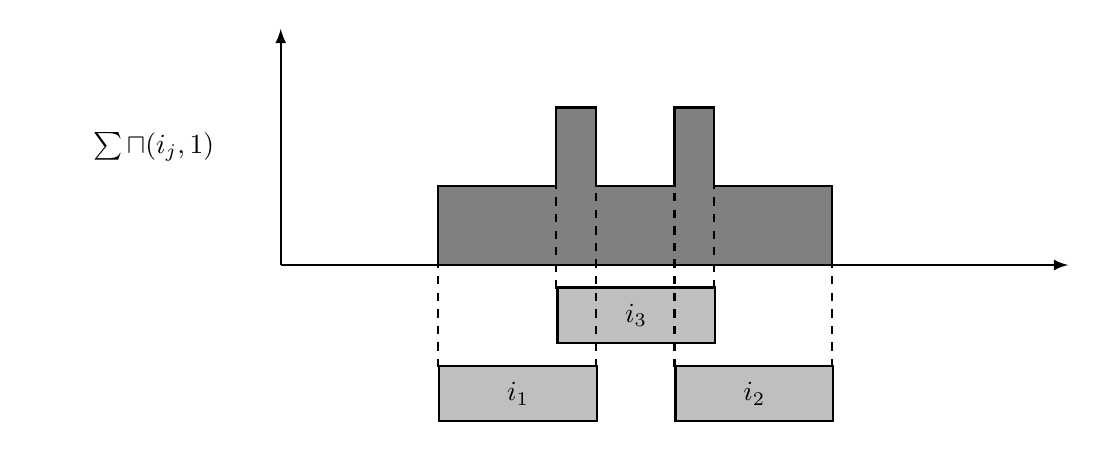
\begin{tikzpicture}
        \draw  (2,1) node[draw, thick, fill=lightgray, rectangle, anchor=south west, inner sep=0pt, minimum width=2cm, minimum height=0.7cm] {\textbf{$i_1$}};
        \draw  (5,1) node[draw, thick, fill=lightgray, rectangle, anchor=south west, inner sep=0pt, minimum width=2cm, minimum height=0.7cm] {\textbf{$i_2$}};
        \draw  (3.5,2) node[draw, thick, fill=lightgray, rectangle, anchor=south west, inner sep=0pt, minimum width=2cm, minimum height=0.7cm] {\textbf{$i_3$}};
        \draw[thick, -latex] (0,3) -- (0,6) node[midway, left, minimum width=3.2cm] {$\sum \sqcap(i_j, 1)$};

        \draw[thick, fill=gray] (2,3) -- (2,4) -- (3.5,4) -- (3.5,5) -- (4,5) -- (4,4) -- (5,4) -- (5,5) -- (5.5,5) -- (5.5,4) -- (7,4) -- (7,3);
        \draw[thick, dashed] (2,1.7) -- (2,3);
        \draw[thick, dashed] (3.5,2.7) -- (3.5,4);
        \draw[thick, dashed] (4,1.7) -- (4,4);
        \draw[thick, dashed] (5,1.7) -- (5,4);
        \draw[thick, dashed] (5.5,2.7) -- (5.5,4);
        \draw[thick, dashed] (7,1.7) -- (7,3);
        \draw[thick, -latex] (0,3) -- (10,3);
    \end{tikzpicture}
}
        \caption{Cumulative functions on $i_1$, $i_2$ and $i_3$ without constraints}
        \label{fig_validation_pulseFunctionNoConst}
    \end{subfigure}\vspace{5mm}
    \begin{subfigure}[b]{\linewidth}
        \centering
        \scalebox{0.9}{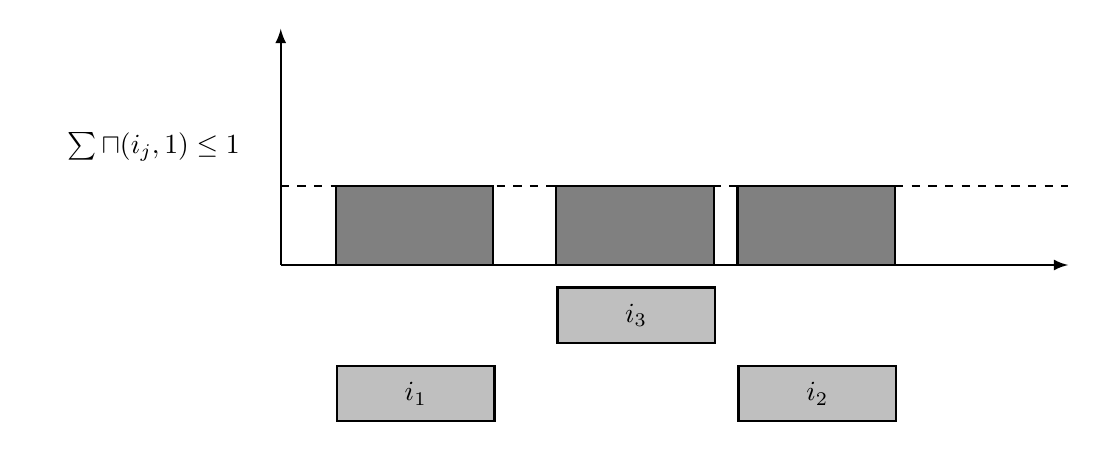
\begin{tikzpicture}
        \draw  (0.7,1) node[draw, thick, fill=lightgray, rectangle, anchor=south west, inner sep=0pt, minimum width=2cm, minimum height=0.7cm] {\textbf{$i_1$}};
        \draw  (5.8,1) node[draw, thick, fill=lightgray, rectangle, anchor=south west, inner sep=0pt, minimum width=2cm, minimum height=0.7cm] {\textbf{$i_2$}};
        \draw  (3.5,2) node[draw, thick, fill=lightgray, rectangle, anchor=south west, inner sep=0pt, minimum width=2cm, minimum height=0.7cm] {\textbf{$i_3$}};
        \draw[thick, -latex] (0,3) -- (0,6) node[midway, left, minimum width=3.2cm] {$\sum \sqcap(i_j, 1) \leq 1$};

        \draw[thick, fill=gray] (0.7,3) -- (0.7,4) -- (2.7,4) -- (2.7,3) -- (3.5,3) -- (3.5,4) -- (5.5,4) -- (5.5,3) -- (5.8,3) -- (5.8,4) -- (7.8,4) -- (7.8,3);
        \draw[thick, dashed] (0,4) -- (10,4);
        \draw[thick, -latex] (0,3) -- (10,3);
    \end{tikzpicture}
}
        \caption{Cumulative functions on $i_1$, $i_2$ and $i_3$ with constraints}
        \label{fig_validation_pulseFunctionWithConst}
    \end{subfigure}
    \caption{Example of three intervals associated with pulse cumulative functions}
    \label{fig_validation_pulseFunction}
\end{figure}

\subsubsection{Cumulative functions}
A \emph{cumulative function} represents the usage of a resource by activities
over time as the sum of their individual contributions. They can be used in
order to constraint the utilization of a resource to remain in a specific
envelope representing the resource's capabilities. While other types of
cumulative functions exist (see~\cite{Laborie08, Laborie09} for further
details), we will use only \emph{pulse} functions throughout this chapter. A
pulse function $\sqcap(i, h)$ increments the usage of a resource by $h$ at the
beginning of interval $i$ and decrements it by $h$ when it completes as shown
in Figure~\ref{fig_validation_pulseFunctionNoConst}.

\subsubsection{Usual constraints on intervals}
Interval variables can usually be constrained using a variety of different
constraints. Among all of those implemented within \CPOpti we use only the
following subset:

\begin{description}

    \item[Presence constraints: ] optional intervals have an attribute $p(i)
        \in [0,1]$ which denotes their presence ($p(i)=1$) or their absence
        ($p(i)=0$) in the final solution. Constraints on $p(i)$ can be used to
        enforce the presence or absence of specific intervals depending on
        configurations. Especially, \emph{alternative} constraints enable to
        force only one interval to be present over a set of intervals. For
        commodity, we will use the $\oplus$ symbol to denote alternative
        constraints defined as follows:
        \begin{displaymath}
            \oplus(I)=1 \Leftrightarrow \underset{i \in I}{\sum} p(i) = 1
        \end{displaymath}
        with $I =  \{ i_1 , \ldots , i_n \}$ a set of optional intervals;

    \item[Precedence constraints: ] intervals can be constrained by precedence
        relations in order to enforce a specific order for their activation. We
        note the precedence constraint operator $ \to $ with the following
        semantics:
        \begin{displaymath}
            i_1 \to i_2 \Leftrightarrow s(i_1) + l(i_1) \leq s(i_2)
        \end{displaymath}

    \item[Cumulative function constraints: ] cumulative functions can be
        constrained in order to maintain the usage of a resource within a
        specific envelope. Figure~\ref{fig_validation_pulseFunctionWithConst}
        shows an example of three intervals associated with pulse cumulative
        functions under a constraint. Here, using pulse functions of height 1
        with a constraint on the cumulative function to be less than 1 actually
        implements a non-overlapping constraint.
\end{description}

\subsection{Problem formulation}
We consider an application $\mathcal{A} = <\tau , \delta>$ following the model
of Section~\ref{sec_systemModel_appModel} and a budget $<\mathcal{N} ,
\mathcal{I} , \mathcal{C} , \mathcal{B} > $ as defined in
Section~\ref{ssec_framework_partitionModel}.

\subsubsection{Job-level solving}
Since intervals apply on jobs and since our task model allows for different
periods in the task set, we will unfold the scheduling over a complete
hyperperiod of length:
\begin{displaymath}
    T_H = \underset{\tau_i \in \tau}{\text{lcm}} (T_i)
\end{displaymath}

We will refer to the k-th activation of task $\tau_i$ as the k-th \emph{job} of
$\tau_i$ denoted $\tau_{i,k}$. Similarly, we will refer to the k-th activation
of the sub-task $\tau_i^j$ as the k-th \emph{sub-job} of $\tau_i^j$ denoted
$\tau_{i,k}^j$. We denote the set of all sub-jobs in a hyperperiod $S$.

Since in our model, precedence relations are only applied to sub-tasks of the
same parent task, we duplicate them to operate at the sub-job level. Moreover,
given the fact that data always have only one producing sub-task, we assume
that each data is over-written every time its producing sub-task is activated.
The k-th production of $\delta_x$ by sub-job $\tau_{i,k}^j$ is denoted
$\delta_{x,k}$.

\subsubsection{Management of I/O requests}
In our application model, sub-tasks are assumed to deal with I/O explicitly.
Requests to read and write to I/O subsystems are modeled as input and output
data in the sub-task. Consequently, I/O requests are not managed differently
from data, the only exception being that data are placed on \PN{} to \PN{}
\PC{}s while I/O requests are assigned to \PN{} to \ION{} (or \ION{} to \PN{})
\PC{}s. 

In the rest of the chapter, and for readability, we will detail how scheduling
data on the \PC{}s is done but we will not explicitly account for the I/O
requests. Yet, the management of I/O requests is strictly equivalent to data
except that the set of eligible \PC{}s to map them is not the same.

\subsubsection{Decision variables}
\label{sssec_validation_decisionVariables}
In our scheduling problem, we have two types of decision variables. 
\begin{description}
    \item[Sub-jobs on \PN{}s:] Each sub-job $\tau_{i,k}^j$ is associated with
        $|\mathcal{N}|$ optional intervals. We note $j(\tau_{i,k}^j , pn_l)$
        the interval variable representing the allocation of sub-job
        $\tau_{i,k}^j$ on the \PN{} $pn_l$. If $j(\tau_{i,k}^j , pn_l)$ is
        present in the final solution, it means that $\tau_{i,k}^j$ is executed
        by \PN{} $pn_l$. The length of each sub-job interval $l(j(\tau_{i,k}^j
        , pn_l))$ is equal to the WCET $C_i^j$ of its corresponding sub-task.
        The activation date and deadline of all intervals are defined by the
        time window $[k \times T_i ; (k+1) \times T_i ]$ during which its
        corresponding sub-job lives. This is represented in
        Figure~\ref{fig_validation_decVarJobs}.

        \begin{figure}
            \centering
            \scalebox{0.9}{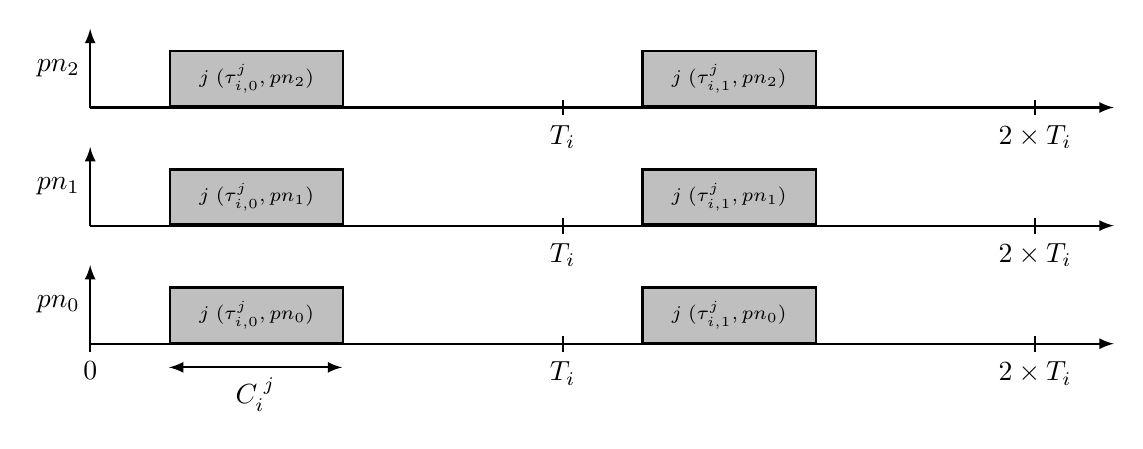
\begin{tikzpicture}
\draw[thick, -latex] (0,0) -- (13,0);
\draw[thick, -latex] (0,1.5) -- (13,1.5);
\draw[thick, -latex] (0,3) -- (13,3);
\draw[thick, -latex] (0,0) -- (0,1) node[midway, left] {$pn_0$};
\draw[thick, -latex] (0,1.5) -- (0,2.5) node[midway, left] {$pn_1$};
\draw[thick, -latex] (0,3) -- (0,4) node[midway, left] {$pn_2$};


\draw  (1,3) node[draw, thick, fill=lightgray, rectangle, anchor=south west, inner sep=0pt, minimum width=2.2cm, minimum height=0.7cm]      {\scriptsize $ j \; ( \tau_{i,0}^j, pn_2 )$};
\draw  (1, 1.5) node[draw, thick, fill=lightgray, rectangle, anchor=south west, inner sep=0pt, minimum width=2.2cm, minimum height=0.7cm]   {\scriptsize $ j \; ( \tau_{i,0}^j, pn_1 )$};
\draw  (1,0) node[draw, thick, fill=lightgray, rectangle, anchor=south west, inner sep=0pt, minimum width=2.2cm, minimum height=0.7cm]      {\scriptsize $ j \; ( \tau_{i,0}^j, pn_0 )$};
\draw[thick, latex-latex] (1,-0.3) -- (3.2,-0.3) node[midway, below] {$C_i^{\; j}$};

\draw[thick] (0,0.1) -- (0, -0.1) node [below] {$0$};
\draw[thick] (6,0.1) -- (6, -0.1) node [below] {$T_i$};
\draw[thick] (6,1.6) -- (6, 1.4) node [below] {$T_i$};
\draw[thick] (6,3.1) -- (6, 2.9) node [below] {$T_i$};


\draw[thick] (12,1.6) -- (12, 1.4) node [below] {$2 \times T_i$};
\draw[thick] (12,0.1) -- (12, -0.1) node [below] {$2 \times T_i$};
\draw[thick] (12,3.1) -- (12, 2.9) node [below] {$2 \times T_i$};

\draw  (7,0) node[draw, thick, fill=lightgray, rectangle, anchor=south west, inner sep=0pt, minimum width=2.2cm, minimum height=0.7cm]      {\scriptsize $ j \; ( \tau_{i,1}^j, pn_0 )$};
\draw  (7, 1.5) node[draw, thick, fill=lightgray, rectangle, anchor=south west, inner sep=0pt, minimum width=2.2cm, minimum height=0.7cm]   {\scriptsize $ j \; ( \tau_{i,1}^j, pn_1 )$};
\draw  (7,3) node[draw, thick, fill=lightgray, rectangle, anchor=south west, inner sep=0pt, minimum width=2.2cm, minimum height=0.7cm]      {\scriptsize $ j \; ( \tau_{i,1}^j, pn_2 )$};
\end{tikzpicture}
}
            \caption{6 interval variables representing 1 sub-task $\tau_i^j$ with 2 sub-jobs that may be scheduled on 3 \PN{}s  }
            \label{fig_validation_decVarJobs}
        \end{figure}

    \item[Data on \PC{}s:] Each data instance $\delta_{x,k}$ is associated with
        $|\mathcal{C}|$ optional interval variables. We note $d(\delta_{x,k} ,
        pc_l)$ the interval representing the allocation of the k-th instance of
        $\delta_x$ on \PC{} $pc_l$. If $d(\delta_{x,k} , pc_l)$ is present in
        the final solution, it means that $\delta_{x,k}$ is sent from the \PN{}
        $src(pc_l)$ to the \PN{} $dst(pc_l)$ via $pc_l$. Counter-intuitively,
        we do not set the length of these intervals to be the time for the data
        to be sent over the NoC. The length of a data interval
        $l(d(\delta_{x,k} , pc_l))$ is set equal to the length $C(pc_l)$ of one
        slot of the \PC{} on which it is sent. The start date $s(d(\delta_{x,k}
        , pc_l))$ of each data interval should be aligned with a slot of its
        corresponding \PC{} $pc_l$ in order to encode the assignment of the
        data transfer during this specific slot. The activation date and
        deadline of a data interval are equal to the living time window $[k
        \times T_i ; (k+1) \times T_i ]$ of its producing sub-job.
\end{description}

\subsection{Constraints}
\subsubsection{Sub-jobs mapping constraints}
Each sub-job must be executed on only one \PN{}. We enforce this behaviour
using constraint~\ref{eq_validation_oneSubjobPerPN}.

\begin{equation}
    \label{eq_validation_oneSubjobPerPN}
    \forall \tau_{i,k}^j \in S ,  
    \oplus(\{ j( \tau_{i,k}^j , pn ) \; | \; \forall pn \in \mathcal{N}\})=1
\end{equation}

If different sub-jobs of the same sub-task could execute on different \PN{}s,
the code and data of the sub-task would need to be duplicated on several
\PN{}s, thus putting a higher pressure on a potentially sensitive resource: the
local SRAM. Moreover, for coherency reason, NoC communication would be required
to transfer static data of the sub-task from one cluster to another, again
putting pressure on a potentially sensitive resource: the NoC. To avoid these
problems, we eliminate sub-task migrations over a hyperperiod by enforcing all
sub-jobs of a sub-task to be assigned to the same \PN{} using
constraint~\ref{eq_validation_allSubjobsSamePN}.

\begin{equation}
    \label{eq_validation_allSubjobsSamePN}
    \forall \tau_{i,k}^j \in S, \; \forall pn \in \mathcal{N}, \;
    p( j( \tau_{i,k}^j, pn )) = p( j( \tau_{i,(k+1) \% \frac{T_H}{T_i}}^j, pn ))
\end{equation}

Figure~\ref{fig_validation_constJobMapping} shows an example of sub-jobs
non-migrating from one cluster to another with intervals on other \PN{}s are
absent.

\begin{figure}
    \centering
    \scalebox{0.9}{\begin{tikzpicture}
                \draw[thick, -latex] (0,0) -- (13,0);
                \draw[thick, -latex] (0,1.5) -- (13,1.5);
                \draw[thick, -latex] (0,3) -- (13,3);
                \draw[thick, -latex] (0,0) -- (0,1) node[midway, left]      {$pn_0$};
                \draw[thick, -latex] (0,1.5) -- (0,2.5) node[midway, left]  {$pn_1$};
                \draw[thick, -latex] (0,3) -- (0,4) node[midway, left] {$pn_2$};
                \draw  (1,3) node[draw, thick, fill=white, pattern=north west lines, rectangle, anchor=south west, inner sep=0pt, minimum width=2.2cm, minimum height=0.7cm] {\scriptsize $ j \; ( \tau_{i,0}^j, pn_2 )$};
                \draw  (1, 1.5) node[draw, thick, fill=lightgray, rectangle, anchor=south west, inner sep=0pt, minimum width=2.2cm, minimum height=0.7cm] {\scriptsize $ j \; ( \tau_{i,0}^j, pn_1 )$};
                \draw  (1,0) node[draw, thick, fill=white, pattern=north west lines, rectangle, anchor=south west, inner sep=0pt, minimum width=2.2cm, minimum height=0.7cm] {\scriptsize $ j \; ( \tau_{i,0}^j, pn_0 )$};
                \draw[thick] (0,0.1) -- (0, -0.1) node [below] {$0$};
                \draw[thick] (6,0.1) -- (6, -0.1) node [below] {$T_i$};
                \draw[thick] (6,1.6) -- (6, 1.4) node [below] {$T_i$};
                \draw[thick] (6,3.1) -- (6, 2.9) node [below] {$T_i$};

                \draw[thick] (12,1.6) -- (12, 1.4) node [below] {$2 \times T_i$};
                \draw[thick] (12,0.1) -- (12, -0.1) node [below] {$2 \times T_i$};
                \draw[thick] (12,3.1) -- (12, 2.9) node [below] {$2 \times T_i$};
                \draw  (7,0) node[draw, thick, fill=white, pattern=north west lines, rectangle, anchor=south west, inner sep=0pt, minimum width=2.2cm, minimum height=0.7cm] {\scriptsize $ j \; ( \tau_{i,1}^j, pn_0 )$};
                \draw  (7, 1.5) node[draw, thick, fill=lightgray, rectangle, anchor=south west, inner sep=0pt, minimum width=2.2cm, minimum height=0.7cm] {\scriptsize $ j \; ( \tau_{i,1}^j, pn_1 )$};
                \draw  (7,3) node[draw, thick, fill=white, pattern=north west lines, rectangle, anchor=south west, inner sep=0pt, minimum width=2.2cm, minimum height=0.7cm] {\scriptsize $ j \; ( \tau_{i,1}^j, pn_2 )$};
    \end{tikzpicture}
}
    \caption{Example of sub-job interval presence following the constraint on
    migration of sub-jobs between \PN{}s }
    \label{fig_validation_constJobMapping}
\end{figure}

\subsubsection{\PN{} utilization constraints}
Since the number of PEs used by one \PN{} is obviously limited, the number of
sub-jobs simultaneously running inside a \PN{} should be limited as well. We
enforce that using cumulative functions as in
constraint~\ref{eq_validation_constPNcoreUtil}.

\begin{equation}
    \label{eq_validation_constPNcoreUtil}
    \forall pn \in \mathcal{N} , \;
    \underset{\forall \tau_{i,k}^j \in S}{\sum} \sqcap( j( \tau_{i,k}^j , pn ),1) \leq N_c(pn)
\end{equation}

Constraint~\ref{eq_validation_constPNcoreUtil} imposes that, at any time, the
number of sub-jobs running concurrently inside one \PN{} never exceeds the
number of PEs of this \PN{}. We argue that such a condition is necessary and
sufficient to ensure that all sub-jobs can always be executed by a PE without
requiring preemption. 

\begin{proof}
    The problem of assigning to each sub-job one PE among $N_c(pn)$ is
    equivalent to a $N_c(pn)$-coloring problem of the associated \emph{Interval
    Graph}. Here, an Interval Graph is a non-weighted non-directed graph having
    sub-jobs for nodes and edges linking all pairs of sub-jobs that overlap in
    time. Such an Interval Graph is well known to be
    \emph{chordal}~\cite{Lekkeikerker1962} and it inherits from all the
    properties of \emph{perfect} graphs. The chromatic number of a perfect
    graph is equal to the size of its largest clique~\cite{Fanica1972}. The
    largest clique of our Interval Graph equals the maximum number of intervals
    that can overlap at any point in time, which is $N_c(pn)$ by design.
    Consequently, our Interval Graph is $N_c(pn)$-colourable, meaning that all
    sub-jobs can be assigned to $N_c(pn)$ PEs without overlapping.
\end{proof}

In addition, the sub-tasks allocated to \PN{}s should meet the memory
specifications of their \PN{}s. This is enforced using
constraint~\ref{eq_validation_constPNmemUtil}. One may note that, in
constraint~\ref{eq_validation_constPNmemUtil}, only the memory footprint of
first sub-job of each sub-task is accounted. Since migration of sub-jobs is
forbidden by constraint~\ref{eq_validation_allSubjobsSamePN}, all sub-jobs of a
sub-task will use the same copy of the code and data.

\begin{equation}
    \label{eq_validation_constPNmemUtil}
    \forall pn \in \mathcal{N} , \;
    \underset{ \tau_i^j \in S }{\sum} p( j( \tau_{i,0}^j , pn ) ) \times M_i^j \leq N_b(pn) \times S_{bank}^{SRAM}
\end{equation}

\subsubsection{Data mapping constraints}
Mapping data on \PC{}s depends on the location of the producing sub-task and
the consuming sub-task(s). If all are located within the same \PN{}, no NoC
transfer is required for the communication since sub-tasks will communicate via
shared memory inside the compute cluster. As long as one consuming sub-task is
assigned to a different cluster from the producing sub-task, then the data must
be sent over a \PC{} connecting the two \PN{}s.
Constraint~\ref{eq_validation_constDataPCmapping} imposes that for the first
produced data interval.

\begin{equation}
    \label{eq_validation_constDataPCmapping}
    \begin{array}{l}
        \forall pc \in \mathcal{C}, \; \forall \delta_{x} \in \delta,  \\
        \hspace{5mm} \Big( \; p(j(prod(\delta_{x,0}), src(pc))) \; \land \underset{\tau_{i,0}^j \in cons(\delta_{x,0})}{\sum} p(j(\tau_{i,0}^j , dst(pc))) \geq 1   \Big)  = p( \delta_{x,0} , pc  ) 
    \end{array}
\end{equation}

In addition, since sub-jobs do not migrate between clusters, every time a data
is produced it should be sent over the same \PC{}s. Consequently, we impose
with constraint~\ref{eq_validation_constDataJobSamePC} that all the data
interval must have a presence attribute equal to those of other data intervals
representing the same data.

\begin{equation}
    \label{eq_validation_constDataJobSamePC}
    \forall pc \in \mathcal{C}, \; \forall \delta_{x,k} \in \delta, \; 
    p( d( \delta_{x,k} , pc ) ) = p( d( \delta_{x,k+1} , pc ) )
\end{equation}

As stated in Section~\ref{sssec_validation_decisionVariables}, start dates of
data intervals must be aligned with a slot of their corresponding \PC{}. We
enforce this using constraint~\ref{eq_validation_constStartDateData}.

\begin{equation}
    \label{eq_validation_constStartDateData}
    \forall pc \in \mathcal{C}, \; \forall \delta_{x,k} \in \delta, \; 
    s( d( \delta_{x,k}, pc ) ) \; \% \; T(pc) = O(pc)
\end{equation}

\subsubsection{\PC{} utilization constraints}
\label{sssec_validation_PCutilConst}
The amount of data that can be transferred during a \PC{} slot must be limited
to meet hardware constraints, and especially the NoC bandwidth and the DMA
capabilities. Our execution model provides a property of collision avoidance on
the NoC, thus drastically simplifying the estimation of NoC transfer durations.
Indeed, using the equations of Section~\ref{ssec_execModel_WCTTNoC}, we can
derive the number of flits required to send each data $\delta_x$ of the
application as $N_{flit}^{total} ( m_x )$ where $m_x$ is the size of
$\delta_x$. In addition, we can derive the number of flits that can safely be
sent during one \PC{} slot from equation~\ref{eq_execModel_NocTransNoConflict}
as:

\begin{displaymath}
    N_{flit}^{PC} (pc) = C(pc) - (R(pc) + 1) \times \Delta_L - R(pc)\times \Delta_S 
\end{displaymath}

Thus, using cumulative functions, we can limit the number of data allocated to
each \PC{} slot so that the number of flits to be sent is less than the
$N_{flit}^{PC} (pc)$. This is enforced using
constraint~\ref{eq_validation_consPcUtilData} and illustrated in
Figure~\ref{fig_validation_consPcUtilData}. 

\begin{equation}
    \label{eq_validation_consPcUtilData}
    \forall pc \in \mathcal{C} , 
    \sum_{\delta_{x,k} \in \delta} \sqcap \Big( d(\delta_{x,k} , pc) , N_{flit}^{total}(m_x) + N_{flit}^{gap} \Big) \leq N_{flit}^{PC} (pc)
\end{equation}

The $N_{flit}^{gap}$ term of equation~\ref{eq_validation_consPcUtilData}
represents the number of empty flits lost in the gap when the DMA jumps from
one contiguous memory area to another. By accounting it for all data, we are
making the conservative assumption that data are placed in non-contiguous
memory areas, thus requiring DMA jumps between all of them. Clearly, computing
the position of data in memory together with the NoC schedule could help
decrease the overhead incurred by these jumps. Indeed, by concatenating data,
larger chunks of memory can be sent efficiently over the NoC, as we recommended
in Section~\ref{sssec_implemExecModel_goodPractices}.
Unfortunately, doing so greatly increases the complexity of the problem which
may thus face limitations regarding scalability. Extending our current model to
include data positioning into the optimization problem in an efficient manner
represents an interesting opportunity of future work.

\begin{figure}
    \centering
    \scalebox{0.9}{   
\newcommand\ttask[7]{\draw  ( #1 , #2 ) node[draw, thick, fill= #3 , rectangle, anchor=south west, inner sep=0pt, minimum width=#4cm, minimum height= #5cm #7] { #6 };}

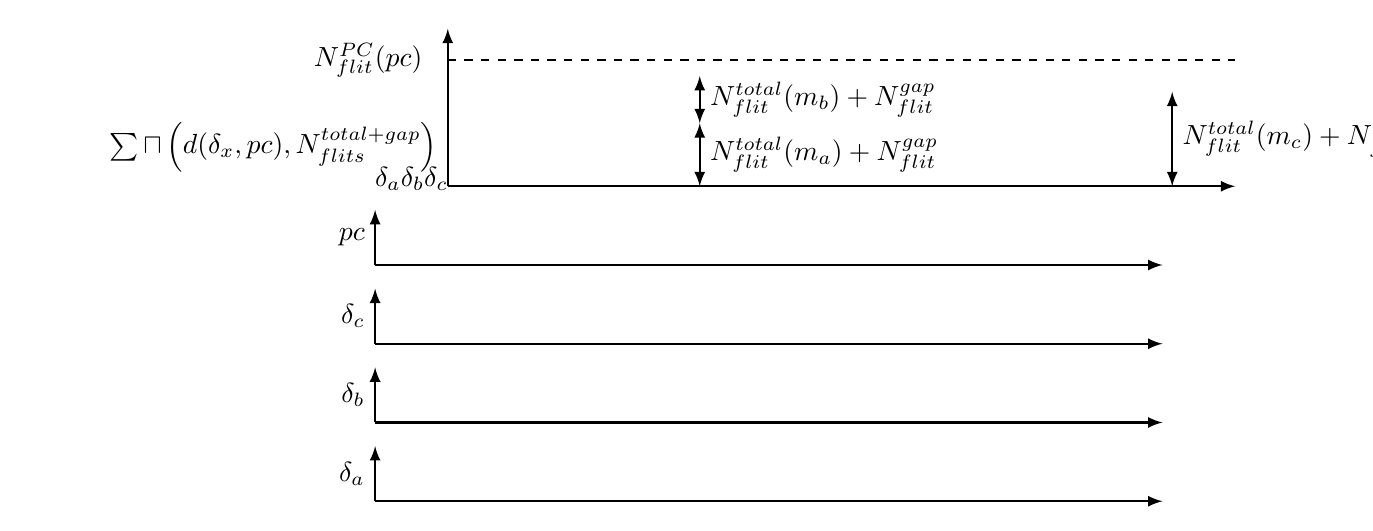
\begin{tikzpicture}
    \draw (12,0) node { };
    \draw[thick, -latex] (0,-1) -- (10,-1);
    \draw[thick, -latex] (0,-1) -- (0,-0.3) node[left, midway] {$pc$};
    \ttask{1}{-1}{gray}{2}{0.5}{}{}
    \ttask{7}{-1}{gray}{2}{0.5}{}{}
    
    \ttask{1}{-2}{}{2}{0.5}{}{, pattern=north west lines}
    \ttask{1}{-3}{}{2}{0.5}{}{, pattern=north west lines}
    \ttask{1}{-4}{}{2}{0.5}{}{, pattern=north west lines}
    \ttask{7}{-2}{}{2}{0.5}{}{, pattern=north west lines}
    \ttask{7}{-3}{}{2}{0.5}{}{, pattern=north west lines}
    \ttask{7}{-4}{}{2}{0.5}{}{, pattern=north west lines}
    
    \draw[thick, -latex] (0,-2) -- (10,-2);
    \draw[thick, -latex] (0,-2) -- (0,-1.3) node[left, midway] {$\delta_c$};
    \draw[thick, -latex] (0,-3) -- (10,-3);
    \draw[thick, -latex] (0,-3) -- (0,-2.3) node[left, midway] {$\delta_b$};
    \draw[thick, -latex] (0,-4) -- (10,-4);
    \draw[thick, -latex] (0,-4) -- (0,-3.3) node[left, midway] {$\delta_a$};
    \ttask{1}{-3}{lightgray}{2}{0.5}{}{}
    \ttask{1}{-4}{lightgray}{2}{0.5}{}{}
    \ttask{7}{-2}{lightgray}{2}{0.5}{}{}
    
    \ttask{1}{0}{lightgray}{2}{0.8}{$\delta_a$}{}
    \ttask{1}{0.8}{lightgray}{2}{0.6}{$\delta_b$}{}
    \ttask{7}{0}{lightgray}{2}{1.2}{$\delta_c$}{} 
    \draw[thick, -latex] (0,0) -- (10,0);
    %\draw[thick, -latex, align=left] (0,0) -- (0,2) node[left, near start] {$\sum \sqcap \left( d(\delta_x,pc) ,\right.$ \\ $ \left. N_{flit}^{total}(m_x) + N_{flit}^{gap}  \right)$};
    \draw[thick, -latex, align=left] (0,0) -- (0,2) node[left, near start] {$\sum \sqcap \left( d(\delta_x,pc) , N_{flits}^{total+gap}  \right)$};
    
    \draw[thick, latex-latex] (3.2, 0) -- (3.2, 0.8) node[midway, right] {$N_{flit}^{total} ( m_a ) + N_{flit}^{gap}$};
    \draw[thick, latex-latex] (3.2, 0.8) -- (3.2, 1.4) node[midway, right] {$N_{flit}^{total} ( m_b ) + N_{flit}^{gap}$};
    \draw[thick, latex-latex] (9.2, 0) -- (9.2, 1.2) node[midway, right] {$N_{flit}^{total} ( m_c ) + N_{flit}^{gap}$};
    
    \draw[thick, dashed] (0, 1.6) -- (10, 1.6);
    \draw (-0.2, 1.6) node[anchor=east] {$N_{flit}^{PC}(pc)$};
\end{tikzpicture}
}
    \caption{Limitation of the amount of data sent during the activation of a
    \PC{} using cumulative functions on data intervals}
    \label{fig_validation_consPcUtilData}
\end{figure}

Since the queues of DMAs can handle only a fixed number of non contiguous
buffers, the number of data to be sent in each \PC{} slot must be limited,
especially because we assume non-contiguous data in memory. This is enforced
using constraint~\ref{eq_validation_consPcUtilDDMA}.

\begin{equation}
    \label{eq_validation_consPcUtilDDMA}
    \forall pc \in \mathcal{C} , 
    \sum_{\delta_{x,k} \in \delta} \sqcap ( d(\delta_{x,k} , pc) , 1 ) \leq N_{bufs}^{DMA}
\end{equation}

\subsubsection{Precedence constraints}
The application model imposes the respect of a set of precedence relations
while executing sub-tasks having the same parent tasks. As explained in
Section~\ref{sec_systemModel_appModel}, only pairs of sub-tasks exchanging data
can be constrained by precedence relations. Consequently, constrained data can
be classified in two categories:
\begin{itemize}
    \item \emph{forward} data are produced by the parent node of the precedence
        relation and consumed by the child node. More formally, assuming a
        precedence $(\tau_i^j , \tau_i^l )$ where $\tau_i^j$ must execute
        before $\tau_i^l$, $\delta_x$ is said to be a forward data if
        $(\tau_i^j = prod(\delta_x)) \land (\tau_i^l \in cons(\delta_x))$;
    \item \emph{backward} data are produced by the child node of the precedence
        relation and consumed by the parent node. In this case, the data
        produced by a sub-job of the child sub-task is consumed during the next
        sub-job of the parent sub-task. More formally, assuming a precedence
        $(\tau_i^j , \tau_i^l )$ where $\tau_i^j$ must execute before
        $\tau_i^l$, $\delta_x$ is said to be a backward data if $(\tau_i^j \in
        cons(\delta_x)) \land (\tau_i^l = prod(\delta_x))$.
\end{itemize}

With forward data, the freshest value semantics imposed by our application
model requires that the child sub-task does not start before it receives the
data produced by the parent sub-task. When both sub-tasks are assigned to the
same \PN{}s, communication is ensured using shared memory. Consequently, the
data produced by the parent sub-task is committed to memory when it completes,
and the child sub-task can start with no delay. This is enforced using
constraint~\ref{eq_validation_constPrecFwSamePN}.

\begin{equation}
    \label{eq_validation_constPrecFwSamePN}
    \forall (\tau_{i,k}^j , \tau_{i,k}^l) \in P_{i,k}, \; \forall pn \in \mathcal{N} , \; 
    j( \tau_{i,k}^j , pn ) \to j( \tau_{i,k}^l , pn )
\end{equation}

However, if the two sub-tasks are assigned different \PN{}s, then a NoC
transfer is required for the produced data to be delivered to the child data.
In order to enforce this precedence between the intervals of the two sub-jobs,
the data interval during which the data is sent over the NoC is used as a
pivot. As shown in Figure~\ref{fig_validation_constFwDataPrec}, two precedence
constraints are used to ensure that the data is sent after the completion of
the parent sub-task (constraint~\ref{eq_validation_constDataProdOrder}) and
before the start of the child sub-task
(constraint~\ref{eq_validation_constDataFwConsumerPrec}). 

\begin{equation}
    \label{eq_validation_constDataProdOrder}
    \forall pc \in \mathcal{C} , \; \forall \delta_{x,k} \in \delta , \;
    j(prod(\delta_{x,k}) , src(pc)) \to d( \delta_{x,k} , pc )   
\end{equation}

\begin{equation}
    \label{eq_validation_constDataFwConsumerPrec}
    \begin{array}{l}
        \forall (\tau_{i,k}^j , \tau_{i,k}^l) \in P_{i,k}, \; \forall pc \in \mathcal{C} , \; \forall \delta_{x,k} \in \delta , \;  \\
        \hspace{5mm} (\tau_{i,k}^j = prod(\delta_{x,k})) \land (\tau_{i,k}^l \in cons(\delta_{x,k})) 
        \Rightarrow d( \delta_{x,k} , pc ) \to j(\tau_{i,k}^l , dst(pc)) 
    \end{array}
\end{equation}

\begin{figure}
    \centering
    \scalebox{0.9}{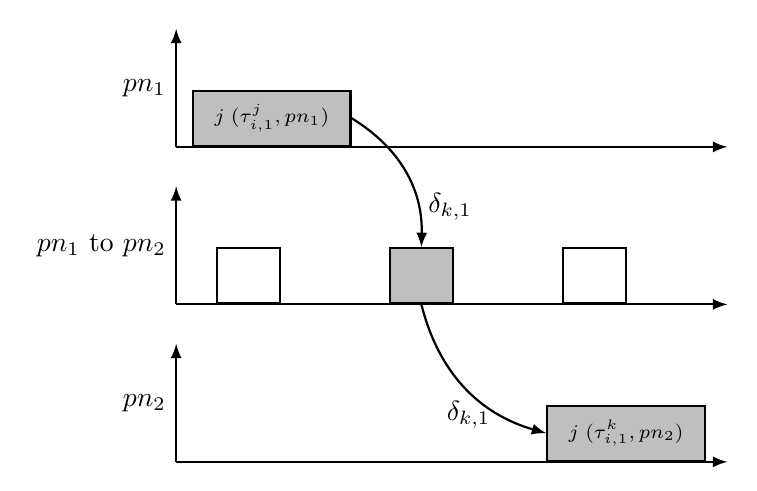
\begin{tikzpicture}
    \draw[thick, -latex] (0,0) -- (7,0); 
    \draw[thick, -latex] (0,2) -- (7,2); 
    \draw[thick, -latex] (0,4) -- (7,4); 
    \draw[thick, -latex] (0,0) -- (0,1.5) node[midway, left] {$pn_2$}; 
    \draw[thick, -latex] (0,2) -- (0,3.5) node[midway, left] {$pn_1$ to $pn_2$}; 
    \draw[thick, -latex] (0,4) -- (0,5.5) node[midway, left] {$pn_1$};

    \draw  (0.2,4) node[draw, thick, fill=lightgray, rectangle, anchor=south west, inner sep=0pt, minimum width=2cm, minimum height=0.7cm] (jpn1) { \scriptsize $ j \; ( \tau_{i,1}^j, pn_1 )$};
    \draw  (4.7,0) node[draw, thick, fill=lightgray, rectangle, anchor=south west, inner sep=0pt, minimum width=2cm, minimum height=0.7cm] (jpn2) { \scriptsize $ j \; ( \tau_{i,1}^k, pn_2 )$};

    \draw  (0.5,2) node[draw, thick, fill=white, rectangle, anchor=south west, inner sep=0pt, minimum width=0.8cm, minimum height=0.7cm] {};
    \draw  (2.7,2) node[draw, thick, fill=lightgray, rectangle, anchor=south west, inner sep=0pt, minimum width=0.8cm, minimum height=0.7cm] (dpc) {};
    \draw  (4.9,2) node[draw, thick, fill=white, rectangle, anchor=south west, inner sep=0pt, minimum width=0.8cm, minimum height=0.7cm] {};
    \draw (jpn1.east) edge[thick, -latex, bend left] node[near end, right] {$\delta_{k,1}$} (dpc.north);
    \draw (dpc.south) edge[thick, -latex, bend right] node[near end, left] {$\delta_{k,1}$} (jpn2.west);
\end{tikzpicture}
}
    \caption{Data interval enforcing the precedence between sub-jobs}
    \label{fig_validation_constFwDataPrec}
\end{figure}

With backward data, the data consumed by the parent sub-job $\tau_{i,k}^j$ is
the data produced by the previous child sub-job $\tau_{i,k-1}^l$. When the two
sub-tasks are assigned the same \PN{},
constraint~\ref{eq_validation_constDataProdOrder} is sufficient to enforce the
correct behaviour. Indeed, the data produced by $\tau_{i,k-1}^l$ is sent after
the completion of the sub-job. Since its deadline equals the deadline of the
producing sub-job, it needs to be sent before the next activation of the task
and thus, necessarily before the activation of $\tau_{i,k}^j$. If the two
sub-tasks are assigned different \PN{}s, we need to ensure that the parent
sub-job ends before the data produced by the child sub-job is sent to ensure
that it never consumes a "too fresh" data. This is enforced using
constraint~\ref{eq_validation_constBwDataPrec}.

\begin{equation}
    \label{eq_validation_constBwDataPrec}
    \begin{array}{l}
        \forall (\tau_{i,k}^j , \tau_{i,k}^l) \in P_{i,k}, \; \forall pc \in \mathcal{C} , \; \forall \delta_{x,k} \in \delta , \;  \\
        \hspace{5mm} (\tau_{i,k}^j \in cons(\delta_{x,k})) \land (\tau_{i,k}^l = prod(\delta_{x,k}))
        \Rightarrow j(\tau_{i,k}^j , dst(pc)) \to d( \delta_{x,k} , pc )  
    \end{array}
\end{equation}


\subsubsection{Determinism constraints}
In our application model, sub-tasks can exchange data, even without being
constrained by precedence relations. So, if a producing and a consuming sub-job
run concurrently, the ordering of the production and consumption of data may
not be deterministic. Indeed, since the time at which the data is produced and
the time at which it is consumed depend on the internal structure of sub-tasks
and on their execution time, the ordering between production and consumption is
not known a priori and may vary at run-time. In this thesis, we consider that
the flexibility of the application model enables to choose any ordering between
production and consumption of data as long as it stays consistent between
execution. To do so, when the two sub-tasks are assigned different \PN{}s, we
avoid the overlapping between the data interval during which the data is sent
and the sub-job interval of the consumer using
constraint~\ref{eq_validation_constDetermDiffPNs}.

\begin{equation}
    \label{eq_validation_constDetermDiffPNs}
    \begin{array}{l}
        \forall \delta_{x,k} \in \delta ,\; \forall \tau_{i,l}^j \in cons( \delta_{x,k} ), \; \forall pc \in \mathcal{C}, \\
        \hspace{5mm} ( prod(\delta_{x,k}), \tau_{i,l}^j ) \notin P_k \land (\tau_{i,l}^j, prod(\delta_{x,k})) \notin P_k \\
        \hspace{5mm} \Rightarrow \sqcap ( d(\delta_{x,k}, pc) ,1) + \sqcap ( j(\tau_{i,l}^j, dst(pc)) ,1) \leq 1
    \end{array}
\end{equation}

Similarly, if the producing and consuming sub-tasks are assigned the same
\PN{}, they should not overlap. This is enforced using
constraint~\ref{eq_validation_constDetermSamePNs}.

\begin{equation}
    \label{eq_validation_constDetermSamePNs}
    \begin{array}{l}
        \forall \delta_{x,k} \in \delta , \; \forall \tau_{i,l}^j \in cons( \delta_{x,k} ), \; \forall pn \in \mathcal{N}, \\
        \hspace{5mm} ( prod(\delta_{x,k}), \tau_{i,l}^j ) \notin P_k \land (\tau_{i,l}^j, prod(\delta_{x,k})) \notin P_k \\
        \hspace{5mm} \Rightarrow \sqcap ( j(prod(\delta_{x,k}), pn) ,1) + \sqcap ( j(\tau_{i,l}^j, pn) ,1) \leq 1
    \end{array}
\end{equation}


\section{Experimental results}
\label{sec_budgetValidation_experimentalRes}

We argue that our CSP formulation of the \emph{Validation} phase can be used
for industrial-sized applications and achieve good performances with realistic
case studies. To demonstrate that, we evaluated the approach over an industrial
case-study provided by Airbus. In the next sections, we will firstly clarify
what should be understood by "good performances" and what our assumptions are
when running the experiments. And secondly, we will analyze several results
from experimental studies and identify the key trade-offs regarding
performance.

\subsection{Goals}
\label{ssec_validation_goalsExpe}
The goal of our experimental study is twofold. Firstly, we aim at showing that
our formal approach is capable of managing large applications as required in an
industrial context. Secondly, we aim at demonstrating that having an automated
and efficient formulation of the problem enables design-space explorations
regarding both budget choices and hypervisor implementations. In order to
investigate all those topics, we will run multiple experiments while varying
three different parameters of the case study.

\subsubsection{Increasing work-load}
In order to demonstrate the ability of our formulation to deal with large and
heavy application, we will not only try to schedule our industrial case study
but we will also modify it in order to artificially increase the work-load to
be processed. By doing so, we show how our CSP formulation can manage not only
existing applications but also more demanding applications as it may be
necessary in the future. 

In order to simulate work-load increase, we will modify the periods of tasks in
the application model. We use a parameter, denoted $k_{div}$ which grows with
the resulting work-load. We will reduce the period of tasks as $\widetilde{T}_i
= \frac{256-k_{div}}{256} \times T_i$ and find out if a schedule can still be
found. With $0 \leq k_{div} \leq 255$, the modified periods can vary between
their original value $T_i$ and $T_i / 256$. Since all other timing parameters
of the application, including the WCET of sub-tasks, are left unmodified,
reducing the period increases the utilization of tasks and simulates a more
demanding application overall. 

\subsubsection{Narrowing the budget}
\label{sssec_validation_expGoalNarrowBudget}
Our formulation of the problem assumes a pre-defined budget in which the
application must be scheduled. Since choosing such a budget does not appear to
be an intuitive task, we will investigate how modifications on an original
budget can impact the resulting performances. Firstly, we will investigate
three different \PN{}s configurations. With $n_{pn}^{orig}$ the original number
of \PN{}s in the budget, we will investigate 3 budgets with $ n_{pn}^{orig}
\leq |\mathcal{N}| \leq n_{pn}^{orig} + 2$ in order to identify how increasing
the number of \PN{}s can impact our capability to find correct schedules. With
a similar idea, we investigate how modifications on \PC{}s can impact
schedulability. With $C_{orig}(pc)$ the original length of a \PC{}, we
investigate three \PC{}s configurations with durations within the $[
    C_{orig}(pc) , C_{orig}(pc) +2 ]$ range for each of them.

\subsubsection{Choosing the DMA configuration}
We explained in Section~\ref{ssection_implemExecModel_systick} how the number
of buffers treated by the DMA can impact the WCET of the hypervisor and thus
the overall performance. Although this value should be fixed in a real avionics
development, we use the opportunity of these experiments to also identify the
trade-off regarding the number of DMA buffers that suits best the needs of our
applications. To do so, we use different values of $N_{bufs}^{DMA}$ in the
$[4,32]$ range to identify which configuration provides the schedulability up
to the highest utilizations.

\subsection{Overview of the case study}
As a case study, we used a \emph{large} industrial application from Airbus.
This application fits in the model of Section~\ref{sec_systemModel_appModel}.
It features several tasks with harmonic periods. In a hyperperiod, the total
number of sub-jobs and data instances is close to 100,000. When turned into
optional intervals, the number of decision variables and constraints in the CSP
grows to several millions. 

In order to run this application, we make several assumptions on the geometry
of its associated budget. These assumptions are detailed below.

\subsubsection{One PE per \PN{}}
In our experiments, we always limited the number of cores of each \PN{} to be
$N_c(pn)=1$. This choice is motivated by the two following reasons:
\begin{enumerate}
    \item assuming only one PE inside each \PN{} enables to eliminate the
        inter-PE interferences at the local SRAM level. Only interferences
        coming from the DMA still need to be taken into account. Consequently,
        WCET of sub-task can be computed accordingly in an efficient manner;
    \item the goal of this thesis is to explore many-core-specific problems
        overall. By avoiding intra-cluster parallelization, we increase the
        need for an efficient inter-cluster parallelization involving a tight
        management of the NoC. Although our CSP formulation is capable of
        managing both intra- and inter-cluster parallelization, we will focus
        only on the latter in order to identify the problems and trade-offs
        that incur with disruptive hardware architectures using NoCs.
\end{enumerate}

\subsubsection{Prompt symmetric \PC{}s}
During our experiments, pairs of \PN{}s in a budget are assumed to be linked
using \emph{prompt} and \emph{symmetric} \PC{}s. We clarify these notions
below.
\begin{description}
    \item[Symmetric] \PC{}s means that in all budgets, all \PC{}s are assumed
        to have identical periods and durations. In addition, all pairs of
        \PN{}s are connected by \PC{}s in both ways. These assumptions simplify
        the expression of budgets and enable an easy generation of many budgets
        following the goals mentioned in
        Section~\ref{ssec_validation_goalsExpe}.
    \item[Prompt ] \PC{}s means that the original duration of a \PC{} (before
        being adjusted as explained in
        Section~\ref{sssec_validation_expGoalNarrowBudget}) is \emph{close} to
        the smallest possible \PC{} duration. The duration of \PC{}s will
        typically be in the order of magnitude of the hypervisor's period and
        the \PC{}s' periods will also be as short as possible.
\end{description}

By using symmetric \PC{}s, we aim at simplifying the automatic expression of
budgets to perform parametric studies and we argue that prompt \PC{}s should
help shorten the delays involved by precedences with forward data. The
evaluation of the CSP under different experimental conditions with different
budgets featuring asymmetric or slow \PC{}s appears as a good opportunity of
future work.



\pgfplotstableread{imgs/tex/dat/validation_expeSpeedups/6_1_8.dat}\kdivvsdurSixUnHuit
\pgfplotstableread{imgs/tex/dat/validation_expeSpeedups/6_1_16.dat}\kdivvsdurSixUnSeize
\pgfplotstableread{imgs/tex/dat/validation_expeSpeedups/6_1_24.dat}\kdivvsdurSixUnVingtquatre
\pgfplotstableread{imgs/tex/dat/validation_expeSpeedups/6_1_32.dat}\kdivvsdurSixUnTrentedeux
\pgfplotstableread{imgs/tex/dat/validation_expeSpeedups/6_2_8.dat}\kdivvsdurSixDeuxHuit
\pgfplotstableread{imgs/tex/dat/validation_expeSpeedups/6_2_16.dat}\kdivvsdurSixDeuxSeize
\pgfplotstableread{imgs/tex/dat/validation_expeSpeedups/6_2_24.dat}\kdivvsdurSixDeuxVingtquatre
\pgfplotstableread{imgs/tex/dat/validation_expeSpeedups/6_2_32.dat}\kdivvsdurSixDeuxTrentedeux
\pgfplotstableread{imgs/tex/dat/validation_expeSpeedups/6_3_8.dat}\kdivvsdurSixTroisHuit
\pgfplotstableread{imgs/tex/dat/validation_expeSpeedups/6_3_16.dat}\kdivvsdurSixTroisSeize
\pgfplotstableread{imgs/tex/dat/validation_expeSpeedups/6_3_24.dat}\kdivvsdurSixTroisVingtquatre
\pgfplotstableread{imgs/tex/dat/validation_expeSpeedups/6_3_32.dat}\kdivvsdurSixTroisTrentedeux
\pgfplotstableread{imgs/tex/dat/validation_expeSpeedups/7_1_8.dat}\kdivvsdurSeptUnHuit
\pgfplotstableread{imgs/tex/dat/validation_expeSpeedups/7_1_16.dat}\kdivvsdurSeptUnSeize
\pgfplotstableread{imgs/tex/dat/validation_expeSpeedups/7_1_24.dat}\kdivvsdurSeptUnVingtquatre
\pgfplotstableread{imgs/tex/dat/validation_expeSpeedups/7_1_32.dat}\kdivvsdurSeptUnTrentedeux
\pgfplotstableread{imgs/tex/dat/validation_expeSpeedups/7_2_8.dat}\kdivvsdurSeptDeuxHuit
\pgfplotstableread{imgs/tex/dat/validation_expeSpeedups/7_2_16.dat}\kdivvsdurSeptDeuxSeize
\pgfplotstableread{imgs/tex/dat/validation_expeSpeedups/7_2_24.dat}\kdivvsdurSeptDeuxVingtquatre
\pgfplotstableread{imgs/tex/dat/validation_expeSpeedups/7_2_32.dat}\kdivvsdurSeptDeuxTrentedeux
\pgfplotstableread{imgs/tex/dat/validation_expeSpeedups/7_3_8.dat}\kdivvsdurSeptTroisHuit
\pgfplotstableread{imgs/tex/dat/validation_expeSpeedups/7_3_16.dat}\kdivvsdurSeptTroisSeize
\pgfplotstableread{imgs/tex/dat/validation_expeSpeedups/7_3_24.dat}\kdivvsdurSeptTroisVingtquatre
\pgfplotstableread{imgs/tex/dat/validation_expeSpeedups/7_3_32.dat}\kdivvsdurSeptTroisTrentedeux
\pgfplotstableread{imgs/tex/dat/validation_expeSpeedups/8_1_8.dat}\kdivvsdurHuitUnHuit
\pgfplotstableread{imgs/tex/dat/validation_expeSpeedups/8_1_16.dat}\kdivvsdurHuitUnSeize
\pgfplotstableread{imgs/tex/dat/validation_expeSpeedups/8_1_24.dat}\kdivvsdurHuitUnVingtquatre
\pgfplotstableread{imgs/tex/dat/validation_expeSpeedups/8_1_32.dat}\kdivvsdurHuitUnTrentedeux
\pgfplotstableread{imgs/tex/dat/validation_expeSpeedups/8_2_8.dat}\kdivvsdurHuitDeuxHuit
\pgfplotstableread{imgs/tex/dat/validation_expeSpeedups/8_2_16.dat}\kdivvsdurHuitDeuxSeize
\pgfplotstableread{imgs/tex/dat/validation_expeSpeedups/8_2_24.dat}\kdivvsdurHuitDeuxVingtquatre
\pgfplotstableread{imgs/tex/dat/validation_expeSpeedups/8_2_32.dat}\kdivvsdurHuitDeuxTrentedeux
\pgfplotstableread{imgs/tex/dat/validation_expeSpeedups/8_3_8.dat}\kdivvsdurHuitTroisHuit
\pgfplotstableread{imgs/tex/dat/validation_expeSpeedups/8_3_16.dat}\kdivvsdurHuitTroisSeize
\pgfplotstableread{imgs/tex/dat/validation_expeSpeedups/8_3_24.dat}\kdivvsdurHuitTroisVingtquatre
\pgfplotstableread{imgs/tex/dat/validation_expeSpeedups/8_3_32.dat}\kdivvsdurHuitTroisTrentedeux
\begin{figure}
    \centering
    \begin{subfigure}[b]{0.3\textwidth} \begin{tikzpicture} \begin{axis}[xscale=0.65,yscale=0.36,xmin=3187500,xmax=48000000,ymin=0,ymax=12000,ytick={0,2000,4000,6000,8000,10000,10800,12000},yticklabels={,,,,,,,},scaled y ticks = false, scaled x ticks = false,, xticklabels=none, legend style={at={(1.5,2.7)},anchor=north east, font=\tiny}]
                \addplot[mark=none, red, dashed, samples=2, domain=3187500:48000000, forget plot] {10800};
                \addplot[mark=*, color=blue] table[x index=0, y index=1]          {\kdivvsdurSixUnHuit};
                \addplot[mark=square*, color=red] table[x index=0, y index=1]     {\kdivvsdurSixUnSeize};
                \addplot[mark=diamond*, color=brown] table[x index=0, y index=1]  {\kdivvsdurSixUnVingtquatre};
                \addplot[mark=triangle*, color=black] table[x index=0, y index=1] {\kdivvsdurSixUnTrentedeux};
                \legend{ $N_{bufs}^{DMA}=8$, $N_{bufs}^{DMA}=16$, $N_{bufs}^{DMA}=24$, $N_{bufs}^{DMA}=32$ }
    \end{axis} \end{tikzpicture} \caption{ $n_{pn}^{orig}$, $C_{orig}(pc)$ } \label{fig_validation_speedupDurationSmallestBudget}
    \end{subfigure}
    \begin{subfigure}[b]{0.3\textwidth} \begin{tikzpicture} \begin{axis}[xscale=0.65,yscale=0.36,xmin=3187500,xmax=48000000,ymin=0,ymax=12000,ytick={0,2000,4000,6000,8000,10000,10800,12000},yticklabels={,,,,,,,},scaled y ticks = false, scaled x ticks = false,, xticklabels=none]
                \addplot[mark=none, red, dashed, samples=2, domain=3187500:48000000, forget plot] {10800};
                \addplot[mark=*, color=blue] table[x index=0, y index=1]          {\kdivvsdurSixDeuxHuit};
                \addplot[mark=square*, color=red] table[x index=0, y index=1]     {\kdivvsdurSixDeuxSeize};
                \addplot[mark=diamond*, color=brown] table[x index=0, y index=1]  {\kdivvsdurSixDeuxVingtquatre};
                \addplot[mark=triangle*, color=black] table[x index=0, y index=1] {\kdivvsdurSixDeuxTrentedeux};
        \end{axis} \end{tikzpicture} \caption{ $n_{pn}^{orig}$, $C_{orig}(pc)+1$ }
    \end{subfigure}
    \begin{subfigure}[b]{0.3\textwidth} \begin{tikzpicture} \begin{axis}[xscale=0.65,yscale=0.36,xmin=3187500,xmax=48000000,ymin=0,ymax=12000,ytick={0,2000,4000,6000,8000,10000,10800,12000},yticklabels={,,,,,,,},scaled y ticks = false, scaled x ticks = false,, xticklabels=none]
                \addplot[mark=none, red, dashed, samples=2, domain=3187500:48000000, forget plot] {10800};
                \addplot[mark=*, color=blue] table[x index=0, y index=1]          {\kdivvsdurSixTroisHuit};
                \addplot[mark=square*, color=red] table[x index=0, y index=1]     {\kdivvsdurSixTroisSeize};
                \addplot[mark=diamond*, color=brown] table[x index=0, y index=1]  {\kdivvsdurSixTroisVingtquatre};
                \addplot[mark=triangle*, color=black] table[x index=0, y index=1] {\kdivvsdurSixTroisTrentedeux};
        \end{axis} \end{tikzpicture} \caption{ $n_{pn}^{orig}$, $C_{orig}(pc)+2$ }
    \end{subfigure}

    \begin{subfigure}[b]{0.3\textwidth} \begin{tikzpicture} \begin{axis}[xscale=0.65,yscale=0.36,xmin=3187500,xmax=48000000,ymin=0,ymax=12000,ytick={0,2000,4000,6000,8000,10000,10800,12000},yticklabels={,,,,,,,},scaled y ticks = false, scaled x ticks = false,, xticklabels=none]
                \addplot[mark=none, red, dashed, samples=2, domain=3187500:48000000, forget plot] {10800};
                \addplot[mark=*, color=blue] table[x index=0, y index=1]          {\kdivvsdurSeptUnHuit};
                \addplot[mark=square*, color=red] table[x index=0, y index=1]     {\kdivvsdurSeptUnSeize};
                \addplot[mark=diamond*, color=brown] table[x index=0, y index=1]  {\kdivvsdurSeptUnVingtquatre};
                \addplot[mark=triangle*, color=black] table[x index=0, y index=1] {\kdivvsdurSeptUnTrentedeux};
        \end{axis} \end{tikzpicture} \caption{ $n_{pn}^{orig}+1$, $C_{orig}(pc)$ } \label{fig_validation_speedupDurationBudget_d}
    \end{subfigure}
    \begin{subfigure}[b]{0.3\textwidth} \begin{tikzpicture} \begin{axis}[xscale=0.65,yscale=0.36,xmin=3187500,xmax=48000000,ymin=0,ymax=12000,ytick={0,2000,4000,6000,8000,10000,10800,12000},yticklabels={,,,,,,,},scaled y ticks = false, scaled x ticks = false,, xticklabels=none]
                \addplot[mark=none, red, dashed, samples=2, domain=3187500:48000000, forget plot] {10800};
                \addplot[mark=*, color=blue] table[x index=0, y index=1]          {\kdivvsdurSeptDeuxHuit};
                \addplot[mark=square*, color=red] table[x index=0, y index=1]     {\kdivvsdurSeptDeuxSeize};
                \addplot[mark=diamond*, color=brown] table[x index=0, y index=1]  {\kdivvsdurSeptDeuxVingtquatre};
                \addplot[mark=triangle*, color=black] table[x index=0, y index=1] {\kdivvsdurSeptDeuxTrentedeux};
        \end{axis} \end{tikzpicture} \caption{ $n_{pn}^{orig}+1$, $C_{orig}(pc)+1$ }
    \end{subfigure}
    \begin{subfigure}[b]{0.3\textwidth} \begin{tikzpicture} \begin{axis}[xscale=0.65,yscale=0.36,xmin=3187500,xmax=48000000,ymin=0,ymax=12000,ytick={0,2000,4000,6000,8000,10000,10800,12000},yticklabels={,,,,,,,},scaled y ticks = false, scaled x ticks = false,, xticklabels=none]
                \addplot[mark=none, red, dashed, samples=2, domain=3187500:48000000, forget plot] {10800};
                \addplot[mark=*, color=blue] table[x index=0, y index=1]          {\kdivvsdurSeptTroisHuit};
                \addplot[mark=square*, color=red] table[x index=0, y index=1]     {\kdivvsdurSeptTroisSeize};
                \addplot[mark=diamond*, color=brown] table[x index=0, y index=1]  {\kdivvsdurSeptTroisVingtquatre};
                \addplot[mark=triangle*, color=black] table[x index=0, y index=1] {\kdivvsdurSeptTroisTrentedeux};
        \end{axis} \end{tikzpicture} \caption{ $n_{pn}^{orig}+1$, $C_{orig}(pc)+2$ }
    \end{subfigure}

    \begin{subfigure}[b]{0.3\textwidth} \begin{tikzpicture} \begin{axis}[xscale=0.65,yscale=0.36,xmin=3187500,xmax=48000000,ymin=0,ymax=12000,ytick={0,2000,4000,6000,8000,10000,10800,12000},yticklabels={,,,,,,,},scaled y ticks = false, scaled x ticks = false,, xticklabels=none]
                \addplot[mark=none, red, dashed, samples=2, domain=3187500:48000000, forget plot] {10800};
                \addplot[mark=*, color=blue] table[x index=0, y index=1]          {\kdivvsdurHuitUnHuit};
                \addplot[mark=square*, color=red] table[x index=0, y index=1]     {\kdivvsdurHuitUnSeize};
                \addplot[mark=diamond*, color=brown] table[x index=0, y index=1]  {\kdivvsdurHuitUnVingtquatre};
                \addplot[mark=triangle*, color=black] table[x index=0, y index=1] {\kdivvsdurHuitUnTrentedeux};
        \end{axis} \end{tikzpicture} \caption{ $n_{pn}^{orig}+2$, $C_{orig}(pc)$ }\label{fig_validation_speedupDurationBudget_g}
    \end{subfigure}
    \begin{subfigure}[b]{0.3\textwidth} \begin{tikzpicture} \begin{axis}[xscale=0.65,yscale=0.36,xmin=3187500,xmax=48000000,ymin=0,ymax=12000,ytick={0,2000,4000,6000,8000,10000,10800,12000},yticklabels={,,,,,,,},scaled y ticks = false, scaled x ticks = false,, xticklabels=none]
                \addplot[mark=none, red, dashed, samples=2, domain=3187500:48000000, forget plot] {10800};
                \addplot[mark=*, color=blue] table[x index=0, y index=1]          {\kdivvsdurHuitDeuxHuit};
                \addplot[mark=square*, color=red] table[x index=0, y index=1]     {\kdivvsdurHuitDeuxSeize};
                \addplot[mark=diamond*, color=brown] table[x index=0, y index=1]  {\kdivvsdurHuitDeuxVingtquatre};
                \addplot[mark=triangle*, color=black] table[x index=0, y index=1] {\kdivvsdurHuitDeuxTrentedeux};
        \end{axis} \end{tikzpicture} \caption{ $n_{pn}^{orig}+2$, $C_{orig}(pc)+1$ }
    \end{subfigure}
    \begin{subfigure}[b]{0.3\textwidth} \begin{tikzpicture} \begin{axis}[xscale=0.65,yscale=0.36,xmin=3187500,xmax=48000000,ymin=0,ymax=12000,ytick={0,2000,4000,6000,8000,10000,10800,12000},yticklabels={,,,,,,,},scaled y ticks = false, scaled x ticks = false,, xticklabels=none]
                \addplot[mark=none, red, dashed, samples=2, domain=3187500:48000000, forget plot] {10800};
                \addplot[mark=*, color=blue] table[x index=0, y index=1]          {\kdivvsdurHuitTroisHuit};
                \addplot[mark=square*, color=red] table[x index=0, y index=1]     {\kdivvsdurHuitTroisSeize};
                \addplot[mark=diamond*, color=brown] table[x index=0, y index=1]  {\kdivvsdurHuitTroisVingtquatre};
                \addplot[mark=triangle*, color=black] table[x index=0, y index=1] {\kdivvsdurHuitTroisTrentedeux};
        \end{axis} \end{tikzpicture} \caption{ $n_{pn}^{orig}+2$, $C_{orig}(pc)+2$ }
    \end{subfigure}

    \caption{Comparison of computation times in function of the load increase with different budgets. The $x$ axis represents the length of the application's hyperperiod (small value means high utilization) and the $y$ axis represents the time used by the solver (timeout at 10,800 seconds)}
    \label{fig_validation_expeSpeedups}
\end{figure}


\subsection{Analysis of results}
Figure~\ref{fig_validation_expeSpeedups} shows the time required by the solver
to produce a solution to the CSP in function of various budgets and DMA
configurations. The $x$ axis represents the hyperperiod on which the
application is scheduled. Short hyperperiods mean high utilization. The $y$
axis represents the time required by the solver to find a solution to the CSP.
A timeout is set to 10,800 seconds, thus explaining the saturation of curves on
the left sides. Reaching the timeout means that no solution has been found and
that the budget, given the application configuration, cannot be considered as
\emph{valid}. On right sides of curves, hyperperiods are longer and finding
solutions can be done more easily, thus validating the intuition that smaller
utilizations lead to better schedulability.
In contrary, it appears clearly in
Figure~\ref{fig_validation_speedupDurationSmallestBudget} that the smallest
budget enables the solver to find solution up to the shortest hyperperiods,
thus reaching the highest utilization ratios. Counter-intuitively, it means
that highest utilization is reached with the smallest number of \PN{}s, and
thus the smallest amount of computational power. One may also note that the
best performances are obtained when the durations of \PC{}s are the smallest
(Figures~\ref{fig_validation_speedupDurationSmallestBudget},
\ref{fig_validation_speedupDurationBudget_d} and
\ref{fig_validation_speedupDurationBudget_g}), while the number of \PN{}s does
not have a clear impact. Based on this, it can be argued that the bottlenecking
parameter in this case study is the NoC delay and not the computational power.
Moreover, while the WCET of the hypervisor was adjusted for each and every of
the four DMA configurations, the impact of the $N_{bufs}^{DMA}$ is not clear.
Moreover, since the raw computational power of \PN{}s does not seem to be a
major issue in this case, it would be interesting as a future work to see
whether relaxing our assumption on the number of PEs allocated to each \PN{}
would help improve the performance. 

We show in Figures~\ref{fig_validation_expePcUtilsSize1}
and~\ref{fig_validation_expePcUtilsSize2} the utilization curves of \PC{}s for
a given schedule produced by the CSP. Each curve depicts the total number of
data that is sent at each activation of each \PC{} slot over a complete
hyperperiod. Figures~\ref{fig_validation_expePcUtilsNbbufs1}
and~\ref{fig_validation_expePcUtilsNbbufs2} show similar curves with the number
of non-contiguous memory areas sent instead of the total size of data. We can
see that curves of Figures~\ref{fig_validation_expePcUtilsSize1}
and~\ref{fig_validation_expePcUtilsSize2} appear to be less busy than
Figures~\ref{fig_validation_expePcUtilsNbbufs1}
and~\ref{fig_validation_expePcUtilsNbbufs2} where the limit imposed by the
constraint~\ref{eq_validation_consPcUtilDDMA} is often reached. Based on this,
we can conclude that the NoC bottleneck of our case study rather comes from the
DMA capability to handle many non-contiguous small data than an actual
limitation due to insufficient bandwidth. As we mentioned in
Section~\ref{sssec_validation_PCutilConst}, optimizing the memory mapping of
data during while computing the mapping and schedule of the application could
help tackle this issue.




%\pgfplotstableread{imgs/tex/dat/validation_expeSpeedups/kdiv_vs_dur_2_6.dat}\kdivvsdurtwosix
%\pgfplotstableread{imgs/tex/dat/validation_expeSpeedups/kdiv_vs_dur_2_7.dat}\kdivvsdurtwoseven
%\pgfplotstableread{imgs/tex/dat/validation_expeSpeedups/kdiv_vs_dur_2_8.dat}\kdivvsdurtwoeight
%\pgfplotstableread{imgs/tex/dat/validation_expeSpeedups/kdiv_vs_dur_3_6.dat}\kdivvsdurthreesix
%\pgfplotstableread{imgs/tex/dat/validation_expeSpeedups/kdiv_vs_dur_3_7.dat}\kdivvsdurthreeseven
%\pgfplotstableread{imgs/tex/dat/validation_expeSpeedups/kdiv_vs_dur_3_8.dat}\kdivvsdurthreeeight
%\pgfplotstableread{imgs/tex/dat/validation_expeSpeedups/kdiv_vs_dur_4_6.dat}\kdivvsdurfoursix
%\pgfplotstableread{imgs/tex/dat/validation_expeSpeedups/kdiv_vs_dur_4_7.dat}\kdivvsdurfourseven
%\pgfplotstableread{imgs/tex/dat/validation_expeSpeedups/kdiv_vs_dur_4_8.dat}\kdivvsdurfoureight
%\begin{figure}
%    \centering
%    \begin{subfigure}[b]{0.3\textwidth} \begin{tikzpicture} \begin{axis}[xscale=0.65,yscale=0.36,xmin=0,xmax=215,ymin=0,ymax=12000,
%                    ytick={0,2000,4000,6000,8000,10000,10800,12000},yticklabels={,,,,,,,},scaled y ticks = false]
%                \addplot[mark=none, red, dashed, samples=2, domain=0:215, forget plot] {10800};
%                \addplot[mark=none, color=black] table[x index=0, y index=1]{\kdivvsdurtwosix};
%        \end{axis} \end{tikzpicture} \caption{ $n_{pn}^{orig}$, $C_{orig}(pc)$ }
%    \end{subfigure}
%    \begin{subfigure}[b]{0.3\textwidth} \begin{tikzpicture} \begin{axis}[xscale=0.65,yscale=0.36,xmin=0,xmax=215,ymin=0,ymax=12000,
%                    ytick={0,2000,4000,6000,8000,10000,10800,12000},yticklabels={,,,,,,,},scaled y ticks = false]
%                \addplot[mark=none, red, dashed, samples=2, domain=0:215, forget plot] {10800};
%                \addplot[mark=none, color=black] table[x index=0, y index=1]{\kdivvsdurtwoseven};
%        \end{axis} \end{tikzpicture} \caption{ $ n_{pn}^{orig} + 1$, $C_{orig}(pc)$ }
%    \end{subfigure}
%    \begin{subfigure}[b]{0.3\textwidth} \begin{tikzpicture} \begin{axis}[xscale=0.65,yscale=0.36,xmin=0,xmax=215,ymin=0,ymax=12000,
%                    ytick={0,2000,4000,6000,8000,10000,10800,12000},yticklabels={,,,,,,,},scaled y ticks = false]
%                \addplot[mark=none, red, dashed, samples=2, domain=0:215, forget plot] {10800};
%                \addplot[mark=none, color=black] table[x index=0, y index=1]{\kdivvsdurtwoeight};
%        \end{axis} \end{tikzpicture} \caption{ $n_{pn}^{orig} + 2$, $C_{orig}(pc)$ }
%    \end{subfigure}
%    \begin{subfigure}[b]{0.3\textwidth} \begin{tikzpicture} \begin{axis}[xscale=0.65,yscale=0.36,xmin=0,xmax=215,ymin=0,ymax=12000,
%                    ytick={0,2000,4000,6000,8000,10000,10800,12000},yticklabels={,,,,,,,},scaled y ticks = false]
%                \addplot[mark=none, red, dashed, samples=2, domain=0:215, forget plot] {10800};
%                \addplot[mark=none, color=black] table[x index=0, y index=1]{\kdivvsdurthreesix};
%        \end{axis} \end{tikzpicture} \caption{ $n_{pn}^{orig}$, $C_{orig}(pc) + 1$ }
%    \end{subfigure}
%    \begin{subfigure}[b]{0.3\textwidth} \begin{tikzpicture} \begin{axis}[xscale=0.65,yscale=0.36,xmin=0,xmax=215,ymin=0,ymax=12000,
%                    ytick={0,2000,4000,6000,8000,10000,10800,12000},yticklabels={,,,,,,,},scaled y ticks = false]
%                \addplot[mark=none, red, dashed, samples=2, domain=0:215, forget plot] {10800};
%                \addplot[mark=none, black] table[x index=0, y index=1]{\kdivvsdurthreeseven};
%        \end{axis} \end{tikzpicture} \caption{ $n_{pn}^{orig} + 1$, $C_{orig}(pc) + 1$ }
%    \end{subfigure}
%    \begin{subfigure}[b]{0.3\textwidth} \begin{tikzpicture} \begin{axis}[xscale=0.65,yscale=0.36,xmin=0,xmax=215,ymin=0,ymax=12000,
%                    ytick={0,2000,4000,6000,8000,10000,10800,12000},yticklabels={,,,,,,,},scaled y ticks = false]
%                \addplot[mark=none, red, dashed, samples=2, domain=0:215, forget plot] {10800};
%                \addplot[mark=none, color=black] table[x index=0, y index=1]{\kdivvsdurthreeeight};
%        \end{axis} \end{tikzpicture} \caption{ $n_{pn}^{orig} + 2$, $C_{orig}(pc) + 1$ }
%    \end{subfigure}
%    \begin{subfigure}[b]{0.3\textwidth} \begin{tikzpicture} \begin{axis}[xscale=0.65,yscale=0.36,xmin=0,xmax=215,ymin=0,ymax=12000,
%                    ytick={0,2000,4000,6000,8000,10000,10800,12000},yticklabels={,,,,,,,},scaled y ticks = false]
%                \addplot[mark=none, red, dashed, samples=2, domain=0:215, forget plot] {10800};
%                \addplot[mark=none, color=black] table[x index=0, y index=1]{\kdivvsdurfoursix};
%        \end{axis} \end{tikzpicture} \caption{ $n_{pn}^{orig}$, $C_{orig}(pc) + 2$ }
%    \end{subfigure}
%    \begin{subfigure}[b]{0.3\textwidth} \begin{tikzpicture} \begin{axis}[xscale=0.65,yscale=0.36,xmin=0,xmax=215,ymin=0,ymax=12000,
%                    ytick={0,2000,4000,6000,8000,10000,10800,12000},yticklabels={,,,,,,,},scaled y ticks = false]
%                \addplot[mark=none, red, dashed, samples=2, domain=0:215, forget plot] {10800};
%                \addplot[mark=none, color=black] table[x index=0, y index=1]{\kdivvsdurfourseven};
%        \end{axis} \end{tikzpicture} \caption{ $n_{pn}^{orig} + 1$, $C_{orig}(pc) + 2$ }
%    \end{subfigure}
%    \begin{subfigure}[b]{0.3\textwidth} \begin{tikzpicture} \begin{axis}[xscale=0.65,yscale=0.36,xmin=0,xmax=215,ymin=0,ymax=12000,
%                    ytick={0,2000,4000,6000,8000,10000,10800,12000},yticklabels={,,,,,,,},scaled y ticks = false]
%                \addplot[mark=none, red, dashed, samples=2, domain=0:215, forget plot] {10800};
%                \addplot[mark=none, color=black] table[x index=0, y index=1]{\kdivvsdurfoureight};
%        \end{axis} \end{tikzpicture} \caption{ $n_{pn}^{orig} + 2$, $C_{orig}(pc) + 2$ }
%    \end{subfigure}
%
%    \caption{Comparison of computation times in function of the load increase with different budgets. The $x$ axis grows with $k_{div}$ and the $y$ axis represents the time used by the solver (timeout at 12,000 seconds)}
%    \label{fig_validation_expeSpeedups}
%\end{figure}







\pgfplotstableread{imgs/tex/dat/validation_expePCutils/PC_0_1_nbbufs.dat}\PCZeroOnenbbufs
\pgfplotstableread{imgs/tex/dat/validation_expePCutils/PC_0_1_size.dat}\PCZeroOnesize
\pgfplotstableread{imgs/tex/dat/validation_expePCutils/PC_0_2_nbbufs.dat}\PCZeroTwonbbufs
\pgfplotstableread{imgs/tex/dat/validation_expePCutils/PC_0_2_size.dat}\PCZeroTwosize
\pgfplotstableread{imgs/tex/dat/validation_expePCutils/PC_0_3_nbbufs.dat}\PCZeroThreenbbufs
\pgfplotstableread{imgs/tex/dat/validation_expePCutils/PC_0_3_size.dat}\PCZeroThreesize
\pgfplotstableread{imgs/tex/dat/validation_expePCutils/PC_0_4_nbbufs.dat}\PCZeroFournbbufs
\pgfplotstableread{imgs/tex/dat/validation_expePCutils/PC_0_4_size.dat}\PCZeroFoursize
\pgfplotstableread{imgs/tex/dat/validation_expePCutils/PC_0_5_nbbufs.dat}\PCZeroFivenbbufs
\pgfplotstableread{imgs/tex/dat/validation_expePCutils/PC_0_5_size.dat}\PCZeroFivesize
\pgfplotstableread{imgs/tex/dat/validation_expePCutils/PC_1_0_nbbufs.dat}\PCOneZeronbbufs
\pgfplotstableread{imgs/tex/dat/validation_expePCutils/PC_1_0_size.dat}\PCOneZerosize
\pgfplotstableread{imgs/tex/dat/validation_expePCutils/PC_1_2_nbbufs.dat}\PCOneTwonbbufs
\pgfplotstableread{imgs/tex/dat/validation_expePCutils/PC_1_2_size.dat}\PCOneTwosize
\pgfplotstableread{imgs/tex/dat/validation_expePCutils/PC_1_3_nbbufs.dat}\PCOneThreenbbufs
\pgfplotstableread{imgs/tex/dat/validation_expePCutils/PC_1_3_size.dat}\PCOneThreesize
\pgfplotstableread{imgs/tex/dat/validation_expePCutils/PC_1_4_nbbufs.dat}\PCOneFournbbufs
\pgfplotstableread{imgs/tex/dat/validation_expePCutils/PC_1_4_size.dat}\PCOneFoursize
\pgfplotstableread{imgs/tex/dat/validation_expePCutils/PC_1_5_nbbufs.dat}\PCOneFivenbbufs
\pgfplotstableread{imgs/tex/dat/validation_expePCutils/PC_1_5_size.dat}\PCOneFivesize
\pgfplotstableread{imgs/tex/dat/validation_expePCutils/PC_2_0_nbbufs.dat}\PCTwoZeronbbufs
\pgfplotstableread{imgs/tex/dat/validation_expePCutils/PC_2_0_size.dat}\PCTwoZerosize
\pgfplotstableread{imgs/tex/dat/validation_expePCutils/PC_2_1_nbbufs.dat}\PCTwoOnenbbufs
\pgfplotstableread{imgs/tex/dat/validation_expePCutils/PC_2_1_size.dat}\PCTwoOnesize
\pgfplotstableread{imgs/tex/dat/validation_expePCutils/PC_2_3_nbbufs.dat}\PCTwoThreenbbufs
\pgfplotstableread{imgs/tex/dat/validation_expePCutils/PC_2_3_size.dat}\PCTwoThreesize
\pgfplotstableread{imgs/tex/dat/validation_expePCutils/PC_2_4_nbbufs.dat}\PCTwoFournbbufs
\pgfplotstableread{imgs/tex/dat/validation_expePCutils/PC_2_4_size.dat}\PCTwoFoursize
\pgfplotstableread{imgs/tex/dat/validation_expePCutils/PC_2_5_nbbufs.dat}\PCTwoFivenbbufs
\pgfplotstableread{imgs/tex/dat/validation_expePCutils/PC_2_5_size.dat}\PCTwoFivesize
\pgfplotstableread{imgs/tex/dat/validation_expePCutils/PC_3_0_nbbufs.dat}\PCThreeZeronbbufs
\pgfplotstableread{imgs/tex/dat/validation_expePCutils/PC_3_0_size.dat}\PCThreeZerosize
\pgfplotstableread{imgs/tex/dat/validation_expePCutils/PC_3_1_nbbufs.dat}\PCThreeOnenbbufs
\pgfplotstableread{imgs/tex/dat/validation_expePCutils/PC_3_1_size.dat}\PCThreeOnesize
\pgfplotstableread{imgs/tex/dat/validation_expePCutils/PC_3_2_nbbufs.dat}\PCThreeTwonbbufs
\pgfplotstableread{imgs/tex/dat/validation_expePCutils/PC_3_2_size.dat}\PCThreeTwosize
\pgfplotstableread{imgs/tex/dat/validation_expePCutils/PC_3_4_nbbufs.dat}\PCThreeFournbbufs
\pgfplotstableread{imgs/tex/dat/validation_expePCutils/PC_3_4_size.dat}\PCThreeFoursize
\pgfplotstableread{imgs/tex/dat/validation_expePCutils/PC_3_5_nbbufs.dat}\PCThreeFivenbbufs
\pgfplotstableread{imgs/tex/dat/validation_expePCutils/PC_3_5_size.dat}\PCThreeFivesize
\pgfplotstableread{imgs/tex/dat/validation_expePCutils/PC_4_0_nbbufs.dat}\PCFourZeronbbufs
\pgfplotstableread{imgs/tex/dat/validation_expePCutils/PC_4_0_size.dat}\PCFourZerosize
\pgfplotstableread{imgs/tex/dat/validation_expePCutils/PC_4_1_nbbufs.dat}\PCFourOnenbbufs
\pgfplotstableread{imgs/tex/dat/validation_expePCutils/PC_4_1_size.dat}\PCFourOnesize
\pgfplotstableread{imgs/tex/dat/validation_expePCutils/PC_4_2_nbbufs.dat}\PCFourTwonbbufs
\pgfplotstableread{imgs/tex/dat/validation_expePCutils/PC_4_2_size.dat}\PCFourTwosize
\pgfplotstableread{imgs/tex/dat/validation_expePCutils/PC_4_3_nbbufs.dat}\PCFourThreenbbufs
\pgfplotstableread{imgs/tex/dat/validation_expePCutils/PC_4_3_size.dat}\PCFourThreesize
\pgfplotstableread{imgs/tex/dat/validation_expePCutils/PC_4_5_nbbufs.dat}\PCFourFivenbbufs
\pgfplotstableread{imgs/tex/dat/validation_expePCutils/PC_4_5_size.dat}\PCFourFivesize
\pgfplotstableread{imgs/tex/dat/validation_expePCutils/PC_5_0_nbbufs.dat}\PCFiveZeronbbufs
\pgfplotstableread{imgs/tex/dat/validation_expePCutils/PC_5_0_size.dat}\PCFiveZerosize
\pgfplotstableread{imgs/tex/dat/validation_expePCutils/PC_5_1_nbbufs.dat}\PCFiveOnenbbufs
\pgfplotstableread{imgs/tex/dat/validation_expePCutils/PC_5_1_size.dat}\PCFiveOnesize
\pgfplotstableread{imgs/tex/dat/validation_expePCutils/PC_5_2_nbbufs.dat}\PCFiveTwonbbufs
\pgfplotstableread{imgs/tex/dat/validation_expePCutils/PC_5_2_size.dat}\PCFiveTwosize
\pgfplotstableread{imgs/tex/dat/validation_expePCutils/PC_5_3_nbbufs.dat}\PCFiveThreenbbufs
\pgfplotstableread{imgs/tex/dat/validation_expePCutils/PC_5_3_size.dat}\PCFiveThreesize
\pgfplotstableread{imgs/tex/dat/validation_expePCutils/PC_5_4_nbbufs.dat}\PCFiveFournbbufs
\pgfplotstableread{imgs/tex/dat/validation_expePCutils/PC_5_4_size.dat}\PCFiveFoursize
\pgfplotstableread{imgs/tex/dat/validation_expePCutils/PC_C0_IO_nbbufs.dat}\PCCZeroIOnbbufs
\pgfplotstableread{imgs/tex/dat/validation_expePCutils/PC_C0_IO_size.dat}\PCCZeroIOsize
\pgfplotstableread{imgs/tex/dat/validation_expePCutils/PC_C1_IO_nbbufs.dat}\PCCOneIOnbbufs
\pgfplotstableread{imgs/tex/dat/validation_expePCutils/PC_C1_IO_size.dat}\PCCOneIOsize
\pgfplotstableread{imgs/tex/dat/validation_expePCutils/PC_C2_IO_nbbufs.dat}\PCCTwoIOnbbufs
\pgfplotstableread{imgs/tex/dat/validation_expePCutils/PC_C2_IO_size.dat}\PCCTwoIOsize
\pgfplotstableread{imgs/tex/dat/validation_expePCutils/PC_C3_IO_nbbufs.dat}\PCCThreeIOnbbufs
\pgfplotstableread{imgs/tex/dat/validation_expePCutils/PC_C3_IO_size.dat}\PCCThreeIOsize
\pgfplotstableread{imgs/tex/dat/validation_expePCutils/PC_C4_IO_nbbufs.dat}\PCCFourIOnbbufs
\pgfplotstableread{imgs/tex/dat/validation_expePCutils/PC_C4_IO_size.dat}\PCCFourIOsize
\pgfplotstableread{imgs/tex/dat/validation_expePCutils/PC_C5_IO_nbbufs.dat}\PCCFiveIOnbbufs
\pgfplotstableread{imgs/tex/dat/validation_expePCutils/PC_C5_IO_size.dat}\PCCFiveIOsize
\pgfplotstableread{imgs/tex/dat/validation_expePCutils/PC_IO_C0_nbbufs.dat}\PCIOCZeronbbufs
\pgfplotstableread{imgs/tex/dat/validation_expePCutils/PC_IO_C0_size.dat}\PCIOCZerosize
\pgfplotstableread{imgs/tex/dat/validation_expePCutils/PC_IO_C1_nbbufs.dat}\PCIOCOnenbbufs
\pgfplotstableread{imgs/tex/dat/validation_expePCutils/PC_IO_C1_size.dat}\PCIOCOnesize
\pgfplotstableread{imgs/tex/dat/validation_expePCutils/PC_IO_C2_nbbufs.dat}\PCIOCTwonbbufs
\pgfplotstableread{imgs/tex/dat/validation_expePCutils/PC_IO_C2_size.dat}\PCIOCTwosize
\pgfplotstableread{imgs/tex/dat/validation_expePCutils/PC_IO_C3_nbbufs.dat}\PCIOCThreenbbufs
\pgfplotstableread{imgs/tex/dat/validation_expePCutils/PC_IO_C3_size.dat}\PCIOCThreesize
\pgfplotstableread{imgs/tex/dat/validation_expePCutils/PC_IO_C4_nbbufs.dat}\PCIOCFournbbufs
\pgfplotstableread{imgs/tex/dat/validation_expePCutils/PC_IO_C4_size.dat}\PCIOCFoursize
\pgfplotstableread{imgs/tex/dat/validation_expePCutils/PC_IO_C5_nbbufs.dat}\PCIOCFivenbbufs
\pgfplotstableread{imgs/tex/dat/validation_expePCutils/PC_IO_C5_size.dat}\PCIOCFivesize



%SIZE

\begin{figure}
    \centering
    \begin{subfigure}[b]{0.3\textwidth} \begin{tikzpicture} \begin{axis}[xmin=0,xmax=140, xscale=0.65,yscale=0.35,ticks=none]
            \addplot[mark=none, color=black] table[x index=0, y index=1] {\PCZeroOnesize};
    \end{axis} \end{tikzpicture} \caption{\PC{} $0$ to $1$} \end{subfigure} 
    \begin{subfigure}[b]{0.3\textwidth} \begin{tikzpicture} \begin{axis}[xmin=0,xmax=140, xscale=0.65,yscale=0.35,ticks=none]
            \addplot[mark=none, color=black] table[x index=0, y index=1] {\PCZeroTwosize};
    \end{axis} \end{tikzpicture} \caption{\PC{} $0$ to $2$} \end{subfigure} 
    \begin{subfigure}[b]{0.3\textwidth} \begin{tikzpicture} \begin{axis}[xmin=0,xmax=140, xscale=0.65,yscale=0.35,ticks=none]
            \addplot[mark=none, color=black] table[x index=0, y index=1] {\PCZeroThreesize};
    \end{axis} \end{tikzpicture} \caption{\PC{} $0$ to $3$} \end{subfigure} 
    \begin{subfigure}[b]{0.3\textwidth} \begin{tikzpicture} \begin{axis}[xmin=0,xmax=140, xscale=0.65,yscale=0.35,ticks=none]
            \addplot[mark=none, color=black] table[x index=0, y index=1] {\PCZeroFoursize};
    \end{axis} \end{tikzpicture} \caption{\PC{} $0$ to $4$} \end{subfigure} 
    \begin{subfigure}[b]{0.3\textwidth} \begin{tikzpicture} \begin{axis}[xmin=0,xmax=140, xscale=0.65,yscale=0.35,ticks=none]
            \addplot[mark=none, color=black] table[x index=0, y index=1] {\PCZeroFivesize};
    \end{axis} \end{tikzpicture} \caption{\PC{} $0$ to $5$} \end{subfigure} 
    \begin{subfigure}[b]{0.3\textwidth} \begin{tikzpicture} \begin{axis}[xmin=0,xmax=140, xscale=0.65,yscale=0.35,ticks=none]
            \addplot[mark=none, color=black] table[x index=0, y index=1] {\PCOneZerosize};
    \end{axis} \end{tikzpicture} \caption{\PC{} $1$ to $0$} \end{subfigure} 
    \begin{subfigure}[b]{0.3\textwidth} \begin{tikzpicture} \begin{axis}[xmin=0,xmax=140, xscale=0.65,yscale=0.35,ticks=none]
            \addplot[mark=none, color=black] table[x index=0, y index=1] {\PCOneTwosize};
    \end{axis} \end{tikzpicture} \caption{\PC{} $1$ to $2$} \end{subfigure} 
    \begin{subfigure}[b]{0.3\textwidth} \begin{tikzpicture} \begin{axis}[xmin=0,xmax=140, xscale=0.65,yscale=0.35,ticks=none]
            \addplot[mark=none, color=black] table[x index=0, y index=1] {\PCOneThreesize};
    \end{axis} \end{tikzpicture} \caption{\PC{} $1$ to $3$} \end{subfigure} 
    \begin{subfigure}[b]{0.3\textwidth} \begin{tikzpicture} \begin{axis}[xmin=0,xmax=140, xscale=0.65,yscale=0.35,ticks=none]
            \addplot[mark=none, color=black] table[x index=0, y index=1] {\PCOneFoursize};
    \end{axis} \end{tikzpicture} \caption{\PC{} $1$ to $4$} \end{subfigure} 
    \begin{subfigure}[b]{0.3\textwidth} \begin{tikzpicture} \begin{axis}[xmin=0,xmax=140, xscale=0.65,yscale=0.35,ticks=none]
            \addplot[mark=none, color=black] table[x index=0, y index=1] {\PCOneFivesize};
    \end{axis} \end{tikzpicture} \caption{\PC{} $1$ to $5$} \end{subfigure} 
    \begin{subfigure}[b]{0.3\textwidth} \begin{tikzpicture} \begin{axis}[xmin=0,xmax=140, xscale=0.65,yscale=0.35,ticks=none]
            \addplot[mark=none, color=black] table[x index=0, y index=1] {\PCTwoZerosize};
    \end{axis} \end{tikzpicture} \caption{\PC{} $2$ to $0$} \end{subfigure} 
    \begin{subfigure}[b]{0.3\textwidth} \begin{tikzpicture} \begin{axis}[xmin=0,xmax=140, xscale=0.65,yscale=0.35,ticks=none]
            \addplot[mark=none, color=black] table[x index=0, y index=1] {\PCTwoOnesize};
    \end{axis} \end{tikzpicture} \caption{\PC{} $2$ to $1$} \end{subfigure} 
    \begin{subfigure}[b]{0.3\textwidth} \begin{tikzpicture} \begin{axis}[xmin=0,xmax=140, xscale=0.65,yscale=0.35,ticks=none]
            \addplot[mark=none, color=black] table[x index=0, y index=1] {\PCTwoThreesize};
    \end{axis} \end{tikzpicture} \caption{\PC{} $2$ to $3$} \end{subfigure} 
    \begin{subfigure}[b]{0.3\textwidth} \begin{tikzpicture} \begin{axis}[xmin=0,xmax=140, xscale=0.65,yscale=0.35,ticks=none]
            \addplot[mark=none, color=black] table[x index=0, y index=1] {\PCTwoFoursize};
    \end{axis} \end{tikzpicture} \caption{\PC{} $2$ to $4$} \end{subfigure} 
    \begin{subfigure}[b]{0.3\textwidth} \begin{tikzpicture} \begin{axis}[xmin=0,xmax=140, xscale=0.65,yscale=0.35,ticks=none]
            \addplot[mark=none, color=black] table[x index=0, y index=1] {\PCTwoFivesize};
    \end{axis} \end{tikzpicture} \caption{\PC{} $2$ to $5$} \end{subfigure} 
    \begin{subfigure}[b]{0.3\textwidth} \begin{tikzpicture} \begin{axis}[xmin=0,xmax=140, xscale=0.65,yscale=0.35,ticks=none]
            \addplot[mark=none, color=black] table[x index=0, y index=1] {\PCThreeZerosize};
    \end{axis} \end{tikzpicture} \caption{\PC{} $3$ to $0$} \end{subfigure} 
    \begin{subfigure}[b]{0.3\textwidth} \begin{tikzpicture} \begin{axis}[xmin=0,xmax=140, xscale=0.65,yscale=0.35,ticks=none]
            \addplot[mark=none, color=black] table[x index=0, y index=1] {\PCThreeOnesize};
    \end{axis} \end{tikzpicture} \caption{\PC{} $3$ to $1$} \end{subfigure} 
    \begin{subfigure}[b]{0.3\textwidth} \begin{tikzpicture} \begin{axis}[xmin=0,xmax=140, xscale=0.65,yscale=0.35,ticks=none]
            \addplot[mark=none, color=black] table[x index=0, y index=1] {\PCThreeTwosize};
    \end{axis} \end{tikzpicture} \caption{\PC{} $3$ to $2$} \end{subfigure} 
    \begin{subfigure}[b]{0.3\textwidth} \begin{tikzpicture} \begin{axis}[xmin=0,xmax=140, xscale=0.65,yscale=0.35,ticks=none]
            \addplot[mark=none, color=black] table[x index=0, y index=1] {\PCThreeFoursize};
    \end{axis} \end{tikzpicture} \caption{\PC{} $3$ to $4$} \end{subfigure} 
    \begin{subfigure}[b]{0.3\textwidth} \begin{tikzpicture} \begin{axis}[xmin=0,xmax=140, xscale=0.65,yscale=0.35,ticks=none]
            \addplot[mark=none, color=black] table[x index=0, y index=1] {\PCThreeFivesize};
    \end{axis} \end{tikzpicture} \caption{\PC{} $3$ to $5$} \end{subfigure} 
    \begin{subfigure}[b]{0.3\textwidth} \begin{tikzpicture} \begin{axis}[xmin=0,xmax=140, xscale=0.65,yscale=0.35,ticks=none]
            \addplot[mark=none, color=black] table[x index=0, y index=1] {\PCFourZerosize};
    \end{axis} \end{tikzpicture} \caption{\PC{} $4$ to $0$} \end{subfigure} 
    \begin{subfigure}[b]{0.3\textwidth} \begin{tikzpicture} \begin{axis}[xmin=0,xmax=140, xscale=0.65,yscale=0.35,ticks=none]
            \addplot[mark=none, color=black] table[x index=0, y index=1] {\PCFourOnesize};
    \end{axis} \end{tikzpicture} \caption{\PC{} $4$ to $1$} \end{subfigure} 
    \begin{subfigure}[b]{0.3\textwidth} \begin{tikzpicture} \begin{axis}[xmin=0,xmax=140, xscale=0.65,yscale=0.35,ticks=none]
            \addplot[mark=none, color=black] table[x index=0, y index=1] {\PCFourTwosize};
    \end{axis} \end{tikzpicture} \caption{\PC{} $4$ to $2$} \end{subfigure} 
    \begin{subfigure}[b]{0.3\textwidth} \begin{tikzpicture} \begin{axis}[xmin=0,xmax=140, xscale=0.65,yscale=0.35,ticks=none]
            \addplot[mark=none, color=black] table[x index=0, y index=1] {\PCFourThreesize};
    \end{axis} \end{tikzpicture} \caption{\PC{} $4$ to $3$} \end{subfigure}
    \caption{Total size of data per \PC{} slot (1/2)}
    \label{fig_validation_expePcUtilsSize1}
\end{figure}

\begin{figure}
    \begin{subfigure}[b]{0.3\textwidth} \begin{tikzpicture} \begin{axis}[xmin=0,xmax=140, xscale=0.65,yscale=0.35,ticks=none]
            \addplot[mark=none, color=black] table[x index=0, y index=1] {\PCFourFivesize};
    \end{axis} \end{tikzpicture} \caption{\PC{} $4$ to $5$} \end{subfigure} 
    \begin{subfigure}[b]{0.3\textwidth} \begin{tikzpicture} \begin{axis}[xmin=0,xmax=140, xscale=0.65,yscale=0.35,ticks=none]
            \addplot[mark=none, color=black] table[x index=0, y index=1] {\PCFiveZerosize};
    \end{axis} \end{tikzpicture} \caption{\PC{} $5$ to $0$} \end{subfigure}
    \centering
    \begin{subfigure}[b]{0.3\textwidth} \begin{tikzpicture} \begin{axis}[xmin=0,xmax=140, xscale=0.65,yscale=0.35,ticks=none]
            \addplot[mark=none, color=black] table[x index=0, y index=1] {\PCFiveOnesize};
    \end{axis} \end{tikzpicture} \caption{\PC{} $5$ to $1$} \end{subfigure} 
    \begin{subfigure}[b]{0.3\textwidth} \begin{tikzpicture} \begin{axis}[xmin=0,xmax=140, xscale=0.65,yscale=0.35,ticks=none]
            \addplot[mark=none, color=black] table[x index=0, y index=1] {\PCFiveTwosize};
    \end{axis} \end{tikzpicture} \caption{\PC{} $5$ to $2$} \end{subfigure} 
    \begin{subfigure}[b]{0.3\textwidth} \begin{tikzpicture} \begin{axis}[xmin=0,xmax=140, xscale=0.65,yscale=0.35,ticks=none]
            \addplot[mark=none, color=black] table[x index=0, y index=1] {\PCFiveThreesize};
    \end{axis} \end{tikzpicture} \caption{\PC{} $5$ to $3$} \end{subfigure} 
    \begin{subfigure}[b]{0.3\textwidth} \begin{tikzpicture} \begin{axis}[xmin=0,xmax=140, xscale=0.65,yscale=0.35,ticks=none]
            \addplot[mark=none, color=black] table[x index=0, y index=1] {\PCFiveFoursize};
    \end{axis} \end{tikzpicture} \caption{\PC{} $5$ to $4$} \end{subfigure} 
    \begin{subfigure}[b]{0.3\textwidth} \begin{tikzpicture} \begin{axis}[xmin=0,xmax=140, xscale=0.65,yscale=0.35,ticks=none]
            \addplot[mark=none, color=black] table[x index=0, y index=1] {\PCCZeroIOsize};
    \end{axis} \end{tikzpicture} \caption{\PC{} $C0$ to $IO$} \end{subfigure} 
    \begin{subfigure}[b]{0.3\textwidth} \begin{tikzpicture} \begin{axis}[xmin=0,xmax=140, xscale=0.65,yscale=0.35,ticks=none]
            \addplot[mark=none, color=black] table[x index=0, y index=1] {\PCCOneIOsize};
    \end{axis} \end{tikzpicture} \caption{\PC{} $C1$ to $IO$} \end{subfigure} 
    \begin{subfigure}[b]{0.3\textwidth} \begin{tikzpicture} \begin{axis}[xmin=0,xmax=140, xscale=0.65,yscale=0.35,ticks=none]
            \addplot[mark=none, color=black] table[x index=0, y index=1] {\PCCTwoIOsize};
    \end{axis} \end{tikzpicture} \caption{\PC{} $C2$ to $IO$} \end{subfigure} 
    \begin{subfigure}[b]{0.3\textwidth} \begin{tikzpicture} \begin{axis}[xmin=0,xmax=140, xscale=0.65,yscale=0.35,ticks=none]
            \addplot[mark=none, color=black] table[x index=0, y index=1] {\PCCThreeIOsize};
    \end{axis} \end{tikzpicture} \caption{\PC{} $C3$ to $IO$} \end{subfigure} 
    \begin{subfigure}[b]{0.3\textwidth} \begin{tikzpicture} \begin{axis}[xmin=0,xmax=140, xscale=0.65,yscale=0.35,ticks=none]
            \addplot[mark=none, color=black] table[x index=0, y index=1] {\PCCFourIOsize};
    \end{axis} \end{tikzpicture} \caption{\PC{} $C4$ to $IO$} \end{subfigure} 
    \begin{subfigure}[b]{0.3\textwidth} \begin{tikzpicture} \begin{axis}[xmin=0,xmax=140, xscale=0.65,yscale=0.35,ticks=none]
            \addplot[mark=none, color=black] table[x index=0, y index=1] {\PCCFiveIOsize};
    \end{axis} \end{tikzpicture} \caption{\PC{} $C5$ to $IO$} \end{subfigure} 
    \begin{subfigure}[b]{0.3\textwidth} \begin{tikzpicture} \begin{axis}[xmin=0,xmax=140, xscale=0.65,yscale=0.35,ticks=none]
            \addplot[mark=none, color=black] table[x index=0, y index=1] {\PCIOCZerosize};
    \end{axis} \end{tikzpicture} \caption{\PC{} $IO$ to $C0$} \end{subfigure} 
    \begin{subfigure}[b]{0.3\textwidth} \begin{tikzpicture} \begin{axis}[xmin=0,xmax=140, xscale=0.65,yscale=0.35,ticks=none]
            \addplot[mark=none, color=black] table[x index=0, y index=1] {\PCIOCOnesize};
    \end{axis} \end{tikzpicture} \caption{\PC{} $IO$ to $C1$} \end{subfigure} 
    \begin{subfigure}[b]{0.3\textwidth} \begin{tikzpicture} \begin{axis}[xmin=0,xmax=140, xscale=0.65,yscale=0.35,ticks=none]
            \addplot[mark=none, color=black] table[x index=0, y index=1] {\PCIOCTwosize};
    \end{axis} \end{tikzpicture} \caption{\PC{} $IO$ to $C2$} \end{subfigure} 
    \begin{subfigure}[b]{0.3\textwidth} \begin{tikzpicture} \begin{axis}[xmin=0,xmax=140, xscale=0.65,yscale=0.35,ticks=none]
            \addplot[mark=none, color=black] table[x index=0, y index=1] {\PCIOCThreesize};
    \end{axis} \end{tikzpicture} \caption{\PC{} $IO$ to $C3$} \end{subfigure} 
    \begin{subfigure}[b]{0.3\textwidth} \begin{tikzpicture} \begin{axis}[xmin=0,xmax=140, xscale=0.65,yscale=0.35,ticks=none]
            \addplot[mark=none, color=black] table[x index=0, y index=1] {\PCIOCFoursize};
    \end{axis} \end{tikzpicture} \caption{\PC{} $IO$ to $C4$} \end{subfigure} 
    \begin{subfigure}[b]{0.3\textwidth} \begin{tikzpicture} \begin{axis}[xmin=0,xmax=140, xscale=0.65,yscale=0.35,ticks=none]
            \addplot[mark=none, color=black] table[x index=0, y index=1] {\PCIOCFivesize};
    \end{axis} \end{tikzpicture} \caption{\PC{} $IO$ to $C5$} \end{subfigure}

    \caption{Total size of data per \PC{} slot (2/2)}
    \label{fig_validation_expePcUtilsSize2}
\end{figure}





% NBBUFS

\begin{figure}
    \centering
    \begin{subfigure}[b]{0.3\textwidth} \begin{tikzpicture} \begin{axis}[xmin=0,xmax=140, xscale=0.65,yscale=0.35,ticks=none]
            \addplot[mark=none, color=black] table[x index=0, y index=1] {\PCZeroOnenbbufs};
    \end{axis} \end{tikzpicture} \caption{\PC{} $0$ to $1$} \end{subfigure} 
    \begin{subfigure}[b]{0.3\textwidth} \begin{tikzpicture} \begin{axis}[xmin=0,xmax=140, xscale=0.65,yscale=0.35,ticks=none]
            \addplot[mark=none, color=black] table[x index=0, y index=1] {\PCZeroTwonbbufs};
    \end{axis} \end{tikzpicture} \caption{\PC{} $0$ to $2$} \end{subfigure} 
    \begin{subfigure}[b]{0.3\textwidth} \begin{tikzpicture} \begin{axis}[xmin=0,xmax=140, xscale=0.65,yscale=0.35,ticks=none]
            \addplot[mark=none, color=black] table[x index=0, y index=1] {\PCZeroThreenbbufs};
    \end{axis} \end{tikzpicture} \caption{\PC{} $0$ to $3$} \end{subfigure} 
    \begin{subfigure}[b]{0.3\textwidth} \begin{tikzpicture} \begin{axis}[xmin=0,xmax=140, xscale=0.65,yscale=0.35,ticks=none]
            \addplot[mark=none, color=black] table[x index=0, y index=1] {\PCZeroFournbbufs};
    \end{axis} \end{tikzpicture} \caption{\PC{} $0$ to $4$} \end{subfigure} 
    \begin{subfigure}[b]{0.3\textwidth} \begin{tikzpicture} \begin{axis}[xmin=0,xmax=140, xscale=0.65,yscale=0.35,ticks=none]
            \addplot[mark=none, color=black] table[x index=0, y index=1] {\PCZeroFivenbbufs};
    \end{axis} \end{tikzpicture} \caption{\PC{} $0$ to $5$} \end{subfigure} 
    \begin{subfigure}[b]{0.3\textwidth} \begin{tikzpicture} \begin{axis}[xmin=0,xmax=140, xscale=0.65,yscale=0.35,ticks=none]
            \addplot[mark=none, color=black] table[x index=0, y index=1] {\PCOneZeronbbufs};
    \end{axis} \end{tikzpicture} \caption{\PC{} $1$ to $0$} \end{subfigure} 
    \begin{subfigure}[b]{0.3\textwidth} \begin{tikzpicture} \begin{axis}[xmin=0,xmax=140, xscale=0.65,yscale=0.35,ticks=none]
            \addplot[mark=none, color=black] table[x index=0, y index=1] {\PCOneTwonbbufs};
    \end{axis} \end{tikzpicture} \caption{\PC{} $1$ to $2$} \end{subfigure} 
    \begin{subfigure}[b]{0.3\textwidth} \begin{tikzpicture} \begin{axis}[xmin=0,xmax=140, xscale=0.65,yscale=0.35,ticks=none]
            \addplot[mark=none, color=black] table[x index=0, y index=1] {\PCOneThreenbbufs};
    \end{axis} \end{tikzpicture} \caption{\PC{} $1$ to $3$} \end{subfigure} 
    \begin{subfigure}[b]{0.3\textwidth} \begin{tikzpicture} \begin{axis}[xmin=0,xmax=140, xscale=0.65,yscale=0.35,ticks=none]
            \addplot[mark=none, color=black] table[x index=0, y index=1] {\PCOneFournbbufs};
    \end{axis} \end{tikzpicture} \caption{\PC{} $1$ to $4$} \end{subfigure} 
    \begin{subfigure}[b]{0.3\textwidth} \begin{tikzpicture} \begin{axis}[xmin=0,xmax=140, xscale=0.65,yscale=0.35,ticks=none]
            \addplot[mark=none, color=black] table[x index=0, y index=1] {\PCOneFivenbbufs};
    \end{axis} \end{tikzpicture} \caption{\PC{} $1$ to $5$} \end{subfigure} 
    \begin{subfigure}[b]{0.3\textwidth} \begin{tikzpicture} \begin{axis}[xmin=0,xmax=140, xscale=0.65,yscale=0.35,ticks=none]
            \addplot[mark=none, color=black] table[x index=0, y index=1] {\PCTwoZeronbbufs};
    \end{axis} \end{tikzpicture} \caption{\PC{} $2$ to $0$} \end{subfigure} 
    \begin{subfigure}[b]{0.3\textwidth} \begin{tikzpicture} \begin{axis}[xmin=0,xmax=140, xscale=0.65,yscale=0.35,ticks=none]
            \addplot[mark=none, color=black] table[x index=0, y index=1] {\PCTwoOnenbbufs};
    \end{axis} \end{tikzpicture} \caption{\PC{} $2$ to $1$} \end{subfigure} 
    \begin{subfigure}[b]{0.3\textwidth} \begin{tikzpicture} \begin{axis}[xmin=0,xmax=140, xscale=0.65,yscale=0.35,ticks=none]
            \addplot[mark=none, color=black] table[x index=0, y index=1] {\PCTwoThreenbbufs};
    \end{axis} \end{tikzpicture} \caption{\PC{} $2$ to $3$} \end{subfigure} 
    \begin{subfigure}[b]{0.3\textwidth} \begin{tikzpicture} \begin{axis}[xmin=0,xmax=140, xscale=0.65,yscale=0.35,ticks=none]
            \addplot[mark=none, color=black] table[x index=0, y index=1] {\PCTwoFournbbufs};
    \end{axis} \end{tikzpicture} \caption{\PC{} $2$ to $4$} \end{subfigure} 
    \begin{subfigure}[b]{0.3\textwidth} \begin{tikzpicture} \begin{axis}[xmin=0,xmax=140, xscale=0.65,yscale=0.35,ticks=none]
            \addplot[mark=none, color=black] table[x index=0, y index=1] {\PCTwoFivenbbufs};
    \end{axis} \end{tikzpicture} \caption{\PC{} $2$ to $5$} \end{subfigure} 
    \begin{subfigure}[b]{0.3\textwidth} \begin{tikzpicture} \begin{axis}[xmin=0,xmax=140, xscale=0.65,yscale=0.35,ticks=none]
            \addplot[mark=none, color=black] table[x index=0, y index=1] {\PCThreeZeronbbufs};
    \end{axis} \end{tikzpicture} \caption{\PC{} $3$ to $0$} \end{subfigure} 
    \begin{subfigure}[b]{0.3\textwidth} \begin{tikzpicture} \begin{axis}[xmin=0,xmax=140, xscale=0.65,yscale=0.35,ticks=none]
            \addplot[mark=none, color=black] table[x index=0, y index=1] {\PCThreeOnenbbufs};
    \end{axis} \end{tikzpicture} \caption{\PC{} $3$ to $1$} \end{subfigure} 
    \begin{subfigure}[b]{0.3\textwidth} \begin{tikzpicture} \begin{axis}[xmin=0,xmax=140, xscale=0.65,yscale=0.35,ticks=none]
            \addplot[mark=none, color=black] table[x index=0, y index=1] {\PCThreeTwonbbufs};
    \end{axis} \end{tikzpicture} \caption{\PC{} $3$ to $2$} \end{subfigure} 
    \begin{subfigure}[b]{0.3\textwidth} \begin{tikzpicture} \begin{axis}[xmin=0,xmax=140, xscale=0.65,yscale=0.35,ticks=none]
            \addplot[mark=none, color=black] table[x index=0, y index=1] {\PCThreeFournbbufs};
    \end{axis} \end{tikzpicture} \caption{\PC{} $3$ to $4$} \end{subfigure} 
    \begin{subfigure}[b]{0.3\textwidth} \begin{tikzpicture} \begin{axis}[xmin=0,xmax=140, xscale=0.65,yscale=0.35,ticks=none]
            \addplot[mark=none, color=black] table[x index=0, y index=1] {\PCThreeFivenbbufs};
    \end{axis} \end{tikzpicture} \caption{\PC{} $3$ to $5$} \end{subfigure} 
    \begin{subfigure}[b]{0.3\textwidth} \begin{tikzpicture} \begin{axis}[xmin=0,xmax=140, xscale=0.65,yscale=0.35,ticks=none]
            \addplot[mark=none, color=black] table[x index=0, y index=1] {\PCFourZeronbbufs};
    \end{axis} \end{tikzpicture} \caption{\PC{} $4$ to $0$} \end{subfigure} 
    \begin{subfigure}[b]{0.3\textwidth} \begin{tikzpicture} \begin{axis}[xmin=0,xmax=140, xscale=0.65,yscale=0.35,ticks=none]
            \addplot[mark=none, color=black] table[x index=0, y index=1] {\PCFourOnenbbufs};
    \end{axis} \end{tikzpicture} \caption{\PC{} $4$ to $1$} \end{subfigure} 
    \begin{subfigure}[b]{0.3\textwidth} \begin{tikzpicture} \begin{axis}[xmin=0,xmax=140, xscale=0.65,yscale=0.35,ticks=none]
            \addplot[mark=none, color=black] table[x index=0, y index=1] {\PCFourTwonbbufs};
    \end{axis} \end{tikzpicture} \caption{\PC{} $4$ to $2$} \end{subfigure} 
    \begin{subfigure}[b]{0.3\textwidth} \begin{tikzpicture} \begin{axis}[xmin=0,xmax=140, xscale=0.65,yscale=0.35,ticks=none]
            \addplot[mark=none, color=black] table[x index=0, y index=1] {\PCFourThreenbbufs};
    \end{axis} \end{tikzpicture} \caption{\PC{} $4$ to $3$} \end{subfigure} 

    \caption{Number of data per \PC{} slot (1/2)}
    \label{fig_validation_expePcUtilsNbbufs1}
\end{figure}

\begin{figure}
    \begin{subfigure}[b]{0.3\textwidth} \begin{tikzpicture} \begin{axis}[xmin=0,xmax=140, xscale=0.65,yscale=0.35,ticks=none]
            \addplot[mark=none, color=black] table[x index=0, y index=1] {\PCFourFivenbbufs};
    \end{axis} \end{tikzpicture} \caption{\PC{} $4$ to $5$} \end{subfigure} 
    \begin{subfigure}[b]{0.3\textwidth} \begin{tikzpicture} \begin{axis}[xmin=0,xmax=140, xscale=0.65,yscale=0.35,ticks=none]
            \addplot[mark=none, color=black] table[x index=0, y index=1] {\PCFiveZeronbbufs};
    \end{axis} \end{tikzpicture} \caption{\PC{} $5$ to $0$} \end{subfigure}
    \centering
    \begin{subfigure}[b]{0.3\textwidth} \begin{tikzpicture} \begin{axis}[xmin=0,xmax=140, xscale=0.65,yscale=0.35,ticks=none]
            \addplot[mark=none, color=black] table[x index=0, y index=1] {\PCFiveOnenbbufs};
    \end{axis} \end{tikzpicture} \caption{\PC{} $5$ to $1$} \end{subfigure} 
    \begin{subfigure}[b]{0.3\textwidth} \begin{tikzpicture} \begin{axis}[xmin=0,xmax=140, xscale=0.65,yscale=0.35,ticks=none]
            \addplot[mark=none, color=black] table[x index=0, y index=1] {\PCFiveTwonbbufs};
    \end{axis} \end{tikzpicture} \caption{\PC{} $5$ to $2$} \end{subfigure} 
    \begin{subfigure}[b]{0.3\textwidth} \begin{tikzpicture} \begin{axis}[xmin=0,xmax=140, xscale=0.65,yscale=0.35,ticks=none]
            \addplot[mark=none, color=black] table[x index=0, y index=1] {\PCFiveThreenbbufs};
    \end{axis} \end{tikzpicture} \caption{\PC{} $5$ to $3$} \end{subfigure} 
    \begin{subfigure}[b]{0.3\textwidth} \begin{tikzpicture} \begin{axis}[xmin=0,xmax=140, xscale=0.65,yscale=0.35,ticks=none]
            \addplot[mark=none, color=black] table[x index=0, y index=1] {\PCFiveFournbbufs};
    \end{axis} \end{tikzpicture} \caption{\PC{} $5$ to $4$} \end{subfigure} 
    \begin{subfigure}[b]{0.3\textwidth} \begin{tikzpicture} \begin{axis}[xmin=0,xmax=140, xscale=0.65,yscale=0.35,ticks=none]
            \addplot[mark=none, color=black] table[x index=0, y index=1] {\PCCZeroIOnbbufs};
    \end{axis} \end{tikzpicture} \caption{\PC{} $C0$ to $IO$} \end{subfigure} 
    \begin{subfigure}[b]{0.3\textwidth} \begin{tikzpicture} \begin{axis}[xmin=0,xmax=140, xscale=0.65,yscale=0.35,ticks=none]
            \addplot[mark=none, color=black] table[x index=0, y index=1] {\PCCOneIOnbbufs};
    \end{axis} \end{tikzpicture} \caption{\PC{} $C1$ to $IO$} \end{subfigure} 
    \begin{subfigure}[b]{0.3\textwidth} \begin{tikzpicture} \begin{axis}[xmin=0,xmax=140, xscale=0.65,yscale=0.35,ticks=none]
            \addplot[mark=none, color=black] table[x index=0, y index=1] {\PCCTwoIOnbbufs};
    \end{axis} \end{tikzpicture} \caption{\PC{} $C2$ to $IO$} \end{subfigure} 
    \begin{subfigure}[b]{0.3\textwidth} \begin{tikzpicture} \begin{axis}[xmin=0,xmax=140, xscale=0.65,yscale=0.35,ticks=none]
            \addplot[mark=none, color=black] table[x index=0, y index=1] {\PCCThreeIOnbbufs};
    \end{axis} \end{tikzpicture} \caption{\PC{} $C3$ to $IO$} \end{subfigure} 
    \begin{subfigure}[b]{0.3\textwidth} \begin{tikzpicture} \begin{axis}[xmin=0,xmax=140, xscale=0.65,yscale=0.35,ticks=none]
            \addplot[mark=none, color=black] table[x index=0, y index=1] {\PCCFourIOnbbufs};
    \end{axis} \end{tikzpicture} \caption{\PC{} $C4$ to $IO$} \end{subfigure} 
    \begin{subfigure}[b]{0.3\textwidth} \begin{tikzpicture} \begin{axis}[xmin=0,xmax=140, xscale=0.65,yscale=0.35,ticks=none]
            \addplot[mark=none, color=black] table[x index=0, y index=1] {\PCCFiveIOnbbufs};
    \end{axis} \end{tikzpicture} \caption{\PC{} $C5$ to $IO$} \end{subfigure} 
    \begin{subfigure}[b]{0.3\textwidth} \begin{tikzpicture} \begin{axis}[xmin=0,xmax=140, xscale=0.65,yscale=0.35,ticks=none]
            \addplot[mark=none, color=black] table[x index=0, y index=1] {\PCIOCZeronbbufs};
    \end{axis} \end{tikzpicture} \caption{\PC{} $IO$ to $C0$} \end{subfigure} 
    \begin{subfigure}[b]{0.3\textwidth} \begin{tikzpicture} \begin{axis}[xmin=0,xmax=140, xscale=0.65,yscale=0.35,ticks=none]
            \addplot[mark=none, color=black] table[x index=0, y index=1] {\PCIOCOnenbbufs};
    \end{axis} \end{tikzpicture} \caption{\PC{} $IO$ to $C1$} \end{subfigure} 
    \begin{subfigure}[b]{0.3\textwidth} \begin{tikzpicture} \begin{axis}[xmin=0,xmax=140, xscale=0.65,yscale=0.35,ticks=none]
            \addplot[mark=none, color=black] table[x index=0, y index=1] {\PCIOCTwonbbufs};
    \end{axis} \end{tikzpicture} \caption{\PC{} $IO$ to $C2$} \end{subfigure} 
    \begin{subfigure}[b]{0.3\textwidth} \begin{tikzpicture} \begin{axis}[xmin=0,xmax=140, xscale=0.65,yscale=0.35,ticks=none]
            \addplot[mark=none, color=black] table[x index=0, y index=1] {\PCIOCThreenbbufs};
    \end{axis} \end{tikzpicture} \caption{\PC{} $IO$ to $C3$} \end{subfigure} 
    \begin{subfigure}[b]{0.3\textwidth} \begin{tikzpicture} \begin{axis}[xmin=0,xmax=140, xscale=0.65,yscale=0.35,ticks=none]
            \addplot[mark=none, color=black] table[x index=0, y index=1] {\PCIOCFournbbufs};
    \end{axis} \end{tikzpicture} \caption{\PC{} $IO$ to $C4$} \end{subfigure} 
    \begin{subfigure}[b]{0.3\textwidth} \begin{tikzpicture} \begin{axis}[xmin=0,xmax=140, xscale=0.65,yscale=0.35,ticks=none]
            \addplot[mark=none, color=black] table[x index=0, y index=1] {\PCIOCFivenbbufs};
    \end{axis} \end{tikzpicture} \caption{\PC{} $IO$ to $C5$} \end{subfigure}

    \caption{Number of data per \PC{} slot (2/2)}
    \label{fig_validation_expePcUtilsNbbufs2}
\end{figure}


\clearpage
\section{Summary}
In this chapter, we detailed how the \emph{Validate} phase of our work-flow can
be implemented using constraint programming. We firstly clarified what our
assumptions on budgets are and provided necessary conditions for budgets to be
valid. Then, we explained how the notion of \emph{Conditional Time-Intervals}
can be used to model our problem and we detailed the actual CSP formulation.
Based on this, we evaluated the capability of our approach for several
different budgets, DMA configurations and application work-loads. By doing so,
we demonstrated that such a formal approach can scale up to industrial-sized
instances of the problem and that the computational power of the platform can
handle heavy work-loads. Yet, we identified the problem of optimizing the
memory mapping of as an interesting challenge to further improve DMA
utilization and our approach overall, thus opening the way to future
contributions.

\clearpage
\subbiblio
\end{document}
